\documentclass[12pt,a4paper]{article}


\usepackage{amsmath}
\usepackage[utf8]{inputenc}
\usepackage{amsmath}
\usepackage{amsfonts}
\usepackage{amssymb}
\usepackage{calrsfs}
\usepackage[left=2cm,right=2cm,top=2cm,bottom=2cm]{geometry}
\usepackage[mathscr]{euscript}
\usepackage{bm}

\usepackage{lmodern}

%%%%%%%strange symbols...%%%
\usepackage{tipa}
%%%%%%%%%%%%%%%%%%%%%%%%%%%

%%%%%%%%%%%attach pdf%%%%%%%%%%%%
\usepackage[final]{pdfpages}
%%%%%%%%%%%%%%%%%%%%%%%%%%%%%%%%%

%%%%%%%%%%for writing symbol above an equality
\newcommand\xeq{\stackrel{\mathclap{\normalfont\mbox{d}}}{=}}
%%%%%%%%%%%%%%%%%%%%%%%%%%%%%%%%%%%%%%%%%%%%

%%%%%For writing large opertors%%%%%%%%%%%
%\usepackage{stmaryrd}
%%%%%%%%%%%%%%%%%%%%%%%%%%%%%%%%%%%%%%%%%%

%%%%%%%%%%for writing large parallel%%%%%%
\usepackage{mathtools}
\DeclarePairedDelimiter\bignorm{\lVert}{\rVert}
%%%%%%%%%%%%%%%%%%%%%%%%%%%%%%%%%%%%%%%%%%

%%%for drawing commutative diagrams.%%%%%%
\usepackage{tikz-cd}  
%%%%%%%%%%%%%%%%%%%%%%%%%%%%%%%%%%%%%%%%%%

%%%%%%%%%%for changing margin
\def\changemargin#1#2{\list{}{\rightmargin#2\leftmargin#1}\item[]}
\let\endchangemargin=\endlist 

\newenvironment{proof}
{\begin{changemargin}{0.5cm}{0.5cm} 
	}%your text here
	{\end{changemargin}
}

\newenvironment{subproof}
{\begin{changemargin}{0.5cm}{0.5cm} 
	}%your text here
	{\end{changemargin}
}

\renewenvironment{i}
{\begin{itemize} 
	}%your text here
	{\end{itemize}
}

\newenvironment{p}
{\begin{proof} 
	}%your text here
	{\end{proof}
}
%%%%%%%%%%%%%%%%%%%%%%%%%%%%%

%%%%%%%%%%%%%%double rules%%%%%%%%%%%%%%%%%%%
\usepackage{lipsum}% Just for this example

\newcommand{\doublerule}[1][.4pt]{%
  \noindent
  \makebox[0pt][l]{\rule[.7ex]{\linewidth}{#1}}%
  \rule[.3ex]{\linewidth}{#1}}
%%%%%%%%%%%%%%%%%%%%%%%%%%%%%%%%%%%%%%%%%%%%%%

\begin{document}
\title{Schramm-Loewner Evolution(SLE)}
\author{Jiwoon Park}
\date{Lent 2019}

\maketitle

\newcommand{\latinmodern}[1]{{\fontfamily{lmss}\selectfont
\textbf{#1}
}}

\newcommand{\thm}{\latinmodern{Theorem) }}
\newcommand{\thmnum}[1]{\latinmodern{Theorem #1) }}
\newcommand{\defi}{\latinmodern{Definition) }}
\newcommand{\definum}[1]{\latinmodern{Definition #1) }}
\newcommand{\lem}{\latinmodern{Lemma) }}
\newcommand{\lemnum}[1]{\latinmodern{Lemma #1) }}
\newcommand{\prop}{\latinmodern{Proposition) }}
\newcommand{\propnum}[1]{\latinmodern{Proposition #1) }}
\newcommand{\corr}{\latinmodern{Corollary) }}
\newcommand{\corrnum}[1]{\latinmodern{Corollary #1) }}
\newcommand{\pf}{\textbf{proof) }}
\newcommand{\fact}{\latinmodern{Fact : }}


\newcommand{\lap}{\triangle} %%Laplacian
\renewcommand{\s}{\vspace{10pt}}
\newcommand{\bull}{$\bullet$}
\newcommand{\sta}{$\star$}
\newcommand{\reals}{\mathbb{R}}

\newcommand{\eop}{\hfill  \textsl{(End of proof)} $\square$} %end of proof
\newcommand{\eos}{\hfill  \textsl{(End of statement)} $\square$} %end of proof
\newcommand{\charac}{\mathrel{\raisebox{0pt}{\scalebox{1}[1]{$1$}} \mkern-5.5mu \raisebox{0.04pt}{\scalebox{1}[1]{$\_$}} \mkern-5.5mu\raisebox{2.3pt}{\scalebox{1}[0.68]{$\bm{|}$}} }}

\newcommand{\call}[1]{\quad \cdots\cdots\cdots\,\,(#1)}

\newcommand{\hh}{\text{\texththeng}}

\newcommand{\norms}[2]{\bignorm[\big]{#1}_{#2}}
\newcommand{\snorms}[2]{\bignorm[\small]{#1}_{#2}}
\newcommand{\abs}[1]{\big| #1 \big|}
\newcommand{\avg}{\mathbb{E}}
\newcommand{\prob}{\mathbb{P}}
\newcommand{\borel}{\mathscr{B}}
\newcommand{\EE}{\mathscr{E}}
\newcommand{\FF}{\mathscr{F}}
\newcommand{\pa}{\partial}
\renewcommand{\H}{\mathbb{H}}
\newcommand{\D}{\mathbb{D}}
\newcommand{\sle}[1]{\text{SLE}_{#1}}

\renewcommand{\vec}{\underline}
\renewcommand{\bar}{\overline}

\def\doubleunderline#1{\underline{\underline{#1}}}

\newcommand{\newday}{\doublerule[0.5pt]}
\newcommand{\digression}{**********************************************************************************************}

\setlength\parindent{0pt}

Website : http://statslab.cam.ac.uk/$\sim$jpmiller/

Pre-requisites : 1. Advanced Probability, 2. Complex Analysis

Co-requisites : Stochastic calculus
\s

\newday

(17th January, Thursday)
\s

\section{Introduction}

SLE is the random, fractal curve which lives in a domain $D\subset \mathbb{C}$. It was introduced in 1999 by Schramm in order to describe the scaling limits of different discrete models. This was a transformative idea in probability because it has led to new hits between probabilistic models and different areas of mathematics.

\s

\textbf{Examples}
\begin{itemize}
\item[1.] \textbf{Loop-erased random walk on $\mathbb{Z}^2$} : Consider a regular random walk $X(n)$ on $\mathbb{Z}^2$, randomly moving particle on the vertices of $\mathbb{Z}^2$ which in each time step goes up/down/left/right with probability 1/4. It's loop-erasure is obtained by erasing the loops that $X(n)$ makes chronologically. The loop-erased random wak is important in probability, in that it builds uniform spanning tree (UST) with Wilson's algorithm.

On the other hand, \emph{Donsker's invariance principle} tells us that $X(n)/\sqrt{n} \rightarrow$two-dimensional BM. The question is, ``What is the scaling limit of the loop-erased of $X$"? This is an $SLE_2$ (proved by Lawler-Schramm-Werner).
\item[2.] \textbf{Percolation on hexagoanl lattice} :
\begin{figure}[h]
\begin{center}
    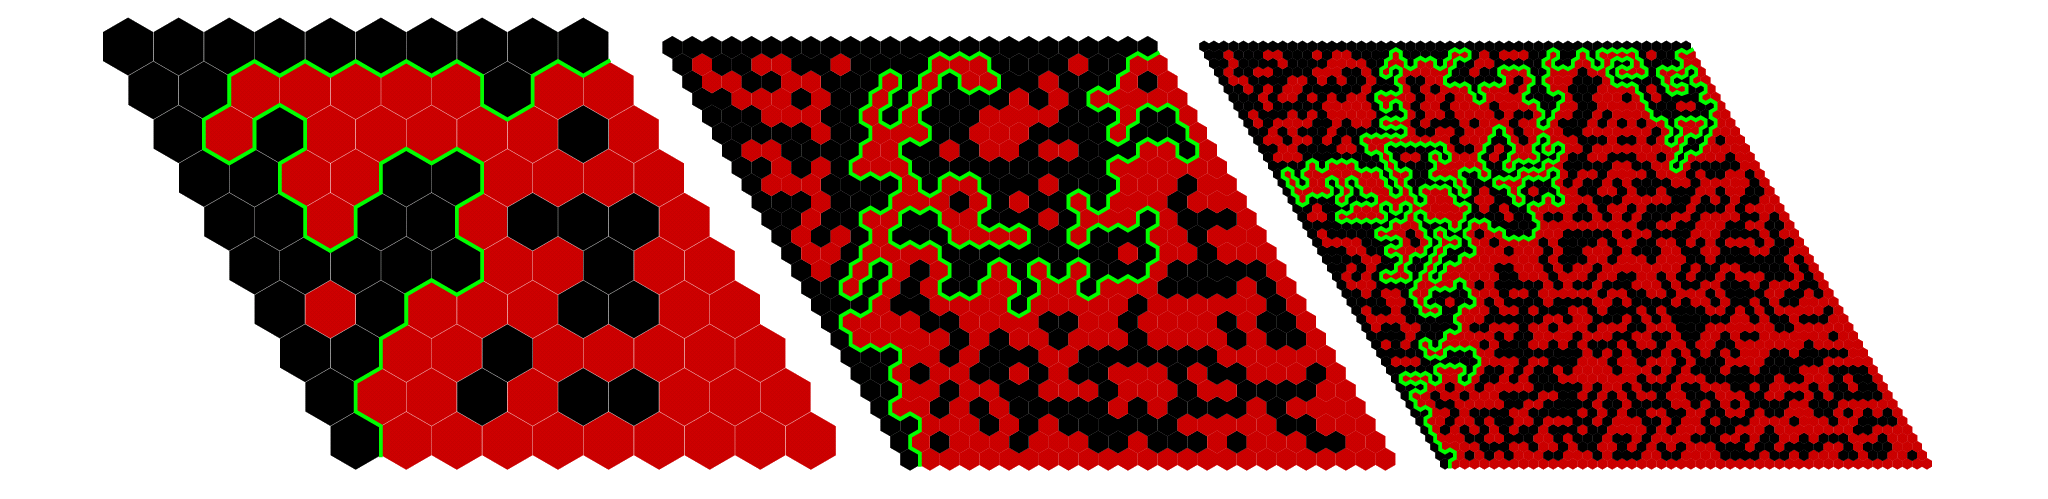
\includegraphics[scale =0.15]{1}
\end{center}
\end{figure}
 Color each hexagon black or white independently each with probability 1/2.
\begin{itemize}
\item[Q.] What is the large-scale behavior of the cluster boundaries?
\item[A.] (Smirnov) They are $SLE_6$. (the proof is not very long, and not very technical)
\end{itemize}
\underline{Famous open question} : prove the same thing on any other planar lattice.
\item[3.] Suppose $X = B_1 + iB_2$, a complex Brownian motion with $B_1, B_2 \sim BM(\reals)$ independent. The \emph{outer boundary} of $X[0,1]$ is the boundary of the unbounded complement of $\mathbb{C} \backslash X[0,1]$.

\underline{Mandelbrot's conjecture} : the ``dimension" of the outer boundary of Brownian motion is 4/3.

This was proved by Lawler-Schramm-Werner using SLE.
\end{itemize}


\subsection{Sturcture}
\begin{itemize}
\item[1.] Will introduce background on complex analysis and define SLE.
\item[2.] Analyze basic properties of SLE, after seeing Ito's formula in Stochastic calculus.
\item[3.] Have a look on more recent devolopments of the subject.
\end{itemize}

\section{Conformal Mappings}

Suppose that $U, V \subset \mathbb{C}$ are domains, $f: U\rightarrow V$ is a map.

\begin{itemize}
\item Then $f$ is \textbf{holomorphic} if $f'(z)=\lim_{w\rightarrow z} (f(w)-f(z))/(w-z)$ exists for all $z\in U$. A map is a \textbf{conformal transformation (or conformal equivalences, or just conformal)} if it is holomorphic and a bijection. 
\item $U\subset \mathbb{C}$ is \textbf{simply connected} if $\mathbb{C}\backslash U$ is connected.
\item Denote unit disk $\mathbb{D} = \{|z|<1\}$, the half plane $\mathbb{H} = \{im(z)>0\}$.
\end{itemize}
\s

\thm \emph{(Riemann mapping theorem)} Suppose $U\subset \mathbb{C}$ is simply connected, $U\neq \mathbb{C}$, $z\in U$. Then there exists a unique conformal transformation $f: \mathbb{D}\rightarrow U$ with $f(0)=z$, $f'(0)\in \reals_{>0}$.
\begin{proof}
\pf You can find the proof of this theorem in any standard complex analysis text. Or, see the extra problem provided at the first example sheet of this course.
\end{proof}
\s

\corr If $U, V\subset \mathbb{C}$ are simply connected, $U, V\neq \mathbb{C}$, $z\in U$, $w\in V$, then there exists a unique conformal transformation $f: U\rightarrow V$ with $f(z)=w$, $f'(0)\in \reals_{>0}$.
\begin{proof}
\pf Map $U, V$ to $\mathbb{D}$ using Riemann mapping theorem. \eop
\end{proof}
\s

\textbf{Important Examples :}
\begin{itemize}
\item[1.] Conformal tranformations of $\mathbb{D} \rightarrow \mathbb{D}$, $U, \mathbb{D}$, $z\in \mathbb{D}$, $f:\mathbb{D}\rightarrow \mathbb{D}$ given by
\begin{align*}
f(w) = \frac{w+z}{1+ \bar{z}w}
\end{align*}
is the unique conformal transformation $\mathbb{D} \rightarrow \mathbb{D}$, $0\mapsto z$, $f'(0)\in \reals_{>0}$.
\s

More generally, every conformal transformation $f: \mathbb{D}\rightarrow \mathbb{D}$ takes the form
\begin{align*}
f(w) = \lambda \frac{w-z}{\bar{z}w-1}, \quad \lambda \in \pa \mathbb{D}, z\in \mathbb{D}
\end{align*}
Note that there are three real parameter family : $\lambda$ has one parameter, $z$ has two parameters. 
\item[2.] The map $\mathbb{H} \rightarrow \mathbb{D}$ given by
\begin{align*}
f(z) = \frac{z-i}{z+i}
\end{align*}
is a conformal transformation, ``Layley transform".
\item[3.] The conformal transformations $\mathbb{H} \rightarrow \mathbb{H}$ are given by
\begin{align*}
f(z) = \frac{az+b}{cz+d}, \quad a,b,c,d\in \reals,\,\, ad-bc=1.
\end{align*}
Note this also has three real parameter family. More generally, there is always a 3-real parameter family of conformal transformations $U\rightarrow V$, for $U, V\subset \mathbb{C}$ simply connected domains.
\end{itemize}

(diagram 2)
$g_t(z)= \sqrt{z^2 + 4t}$ maps $\mathbb{H}\backslash[0, 2\sqrt{t}i] \rightarrow \mathbb{H}$. Note
\begin{align*}
\pa_t g_t(z) = \frac{4}{2\sqrt{z^2 + 4t}} = \frac{2}{g_t(z)}
\end{align*}
so $(g_t)$ is described by the ODE : $\pa_t g_t(z) = 2/g_t(z)$, $g_0(z)=z$.
\s

\textbf{Loewner's theorem :} Suppose $\gamma$ is a curve in $\mathbb{H}$ with $\gamma(0)=0$ and is simple. Suppose there is a uniuqe conformal transformation $g_t : \mathbb{H} \backslash \gamma[0,t] \rightarrow \mathbb{H}$ with $g_t(z)- z\rightarrow 0$ as $z\rightarrow \infty$. Then
\begin{align*}
\pa_t g_t(z) = \frac{2}{g_t(z) - u_t}
\end{align*}
where $u_t$ is a continuous $\reals$-valued function.
\s

$SLE_t \leftrightarrow u_t = \sqrt{\kappa} B_t$, $t>0$, $B$ is a standard BM.
\s

\newday

(22nd January, Tuesday)
\s

Last time : conformal transformations, Reimann mapping theorem.
\s

\textbf{Important example :} For each $t\geq 0$, let $\H_t =\H \backslash [0, 2i\sqrt{t}]$. Let $g_t: \H_t \rightarrow \H$ be the map $z\mapsto \sqrt{z^2 + 4t}$. Then $g_t$ has the following properties.
\begin{i}
\item[1.] $g_t$ has the special property that $|g_t(z) - z| \rightarrow 0$ as $|z| \rightarrow \infty$. That is ``$g_t$ looks like the identity map at $\infty$".
\item[2.] $\pa_t g_t(z) = \frac{2}{g_t(z)}$, $g_0(z) = z$. So $(g_t(z))$ solves the ODE
\begin{align*}
\pa_t = \frac{2}{g_t(z)}, \quad g_0(z) = z \quad \cdots\cdots\cdots (\star)
\end{align*}
For each $z\in \H$, $(\star)$ has a unique solution up until $\tau(z) = \inf \{t\geq 0: |g_t(z)|=0 \}$. The maps $(g_t)$ are characterized by $(\star)$.
\s

\textbf{Idea :} The ODE $(\star)$ encods the curve $\gamma(t) = 2\sqrt{t} i$. (Conversely, given the curve, this parametrization is the one that makes the characterizing ODE $(\star)$ nice)
\end{i}
\s
 
\textbf{Preview :} Suppose $\gamma$ is a simple curve in $\H$ with $\gamma(0)=0$. For each $t\geq 0$, let $g_t$ be the unique conformal transformation $\H_t \rightarrow \H$ with $|g_t(z)- z| \rightarrow 0$ as $z\rightarrow \infty$. \emph{[Will prove existence/uniqueness of such a map later]} Then there exists continuous $\reals$-values function $w$ such that
\begin{align*}
\pa_t g_t(z) = \frac{2}{g_t(z) - w_t}, \quad g_0(z) =z
\end{align*}
This is called the \textbf{Chordal Loewner equation}. We also have a correspondence
\begin{align*}
\text{Curves } \gamma \quad \leftrightarrow \quad \reals-\text{valued, continuous functions } w
\end{align*}
As noted earlier, the example above corresponds to $w\equiv 0$ and $SLE_{\kappa}$ corresponds to $w_z = \sqrt{\kappa} B_t$ for $\kappa \geq 0$, $B$ a standard Brownian motion.
\s

\section*{Brownian Motion, Conformal Maps, Harmonic Functions}

\defi A \textbf{complex Brownian motion} $B_t$ started from $z\in \mathbb{C}$ is a process of the form $B_t = B_t^1 + iB_t^2$ where $B^1$, $B^2$ are independent standard Brownian motions with $B_0 =z$. 
\s

These are objects intimately connected with harmonis functions and conformal maps.
\s

\textbf{Recall :} $f= u + iv : \mathbb{C}_{x,y} \rightarrow \mathbb{C}_{u,v}$ is holomorphic \emph{iff} $u,v$ solve the \emph{Cauchy-Riemann equations}
\begin{align*}
\frac{\pa u}{\pa x} = \frac{\pa v}{\pa y}, \quad \frac{\pa u}{\pa y} = - \frac{\pa v}{\pa x}
\end{align*}
\textit{Consequence :} $f$ is holomorphic, then $u,v$ are harmoic, \textit{i.e.} $\lap u = \lap v=0$.
\s

In \emph{Advanced $\prob$}, we saw that harmonic functions and Brownian motions are closely related. 
\s

\thm Let $u$ be a harmonic function on a bounded domain $D\subset \mathbb{C}$ which is continuous on $\overline{D}$. Let $\prob_z$ be the law of a complex Brownian motion starting from $z\in D$ and $\tau = \inf \{ t\geq 0 : B_t \not\in D \}$. Then :
\begin{align*}
u(z) = \avg_z [u(B_{\tau})]
\end{align*}
\begin{p}
\pf Saw in \emph{Advnced probability.} Will see another proof in \emph{Stochastic Calculus} using It\^o's formula.
\end{p}
\s

The following two theorems are a good characterization of harmonic functions.(These properties are also true in higher dimensions, but we do not need those results for this course.)
\s

\thm \emph{(Mean-value property)} In the setting of the pervious theorem, if $z\in D$, $r>0$, so that $B(z,r)\subset D$, then
\begin{align*}
u(z) = \frac{1}{2\pi} \int_0^{\pi} u(z + re^{i\theta}) d\theta
\end{align*}
\begin{p}
\pf Apply the previous theorem with $D= B(z,r)$ and $u$ restrited to $B(z,r)$. Use that the first exit distribution of a complex $BM$ from $B(z,r)$ starting from $z$ is uniform on the circle $\pa B(z,r)$.

\eop
\end{p}
\s

\thm \emph{(Maximum principle)} Suppose that $u$ is harmonic on a domain $D\subset \mathbb{C}$. If $u$ attains its maximum at an inteiror point $z_0$ then $u$ is constant.
\begin{p}
\pf Let $D_0 = \{z\in D : u(z) = u(z_0) \}$. Then $D_0 \neq \phi$ as $z_0 \in D$. Since $u$ is continuous, $D_0$ is closed. By the mean-value property, $D_0$ is open. Therefore, $D=D_0$.

\eop
\end{p}
\s

As a consequence, we obtain a similar principle for holomorphic functions.
\s

\thm \emph{(Maximum modulus principle)} Let $D\subset \mathbb{C}$ be a domain, $f: D\rightarrow \mathbb{C}$ be holomorphic. If $|f|$ attains its maximum at an interior point, then $f$ is constant.
\begin{p}
\pf Let $K\subset D$ be compact. By replacing $f$ with $f+M$ for $M>0$ sufficiently large, we can assume wlog that $|f|\neq 0$ on $K$. Note that $\log |f| = \Re (\log f)$ is harmonic on $K$. If $|f|$ attians its maximum on $K$, then so does $\log |f|$. Hence $\log |f|$ is constant on $K$ and therefore so is $|f|$. Since $K\subset D$ was arbitrary, if $|f|$ has an interior maximum then $|f|$ is constant on $D$. So $\text{area}(f(D))$ =0.

\quad But If $\exists sz\in D$ with $f'(z) \neq 0$, then $f'(w) \neq 0$ for $w$ in a neighbourhood of $z$. So
\begin{align*}
\int |f'(w)|^2 > 0 \quad \Rightarrow \quad \text{area}(f(D))>0, 
\end{align*}
a contardiction.

\eop
\end{p}
\s

Let us conclude our review of complex analysis with an important lemma.
\s

\textbf{Schwarz lemma :} Suppose $f: \mathbb{D} \rightarrow \mathbb{D}$ is holomorphic with $f(0)=0$. Then $|f(z)| \leq |z|$ for all $z\in \mathbb{D}$. If $|f(z)| = |z|$ for some $z\in \mathbb{D} \backslash\{0\}$, then $f(w) = e^{i\theta} w$ for some $\theta \in \reals$. \textit{i.e.} $f$ is just a rotation.
\begin{p}
\pf Let
\begin{align*}
g(w) = \begin{cases}
f(w) /w \quad \text{if } w\neq 0 \\
f'(0) \quad \text{if } w = 0
\end{cases}
\end{align*}
Then $g$ is holomorphic, $|g(w)|\leq 1$ for all $w\in \mathbb{D}$. By the maximum modulus principle, $|f(w)| \leq |w|$. If $|f(z)|= |z|$ for some $z\in \mathbb{D} \backslash \{0\}$, then $g$ is constant, and therefore $f(w) = e^{i\theta} w$ for some $\theta \in \reals$.

\eop
\end{p}

\newday

(24th January, Thursday)
\s

\subsection*{Distortion estimates for conformal maps}

Let $U = \{$conformal transformations $f: \mathbb{D} \rightarrow D \}$ where $D\subset \mathbb{C}$, $D\neq \mathbb{C}$, $0\in D$, $f(0)=0$, $f'(0)=1$.
\s

\thm \emph{(Koebe-1/4)} If $f\in U$ and $0<r\leq 1$, then $B(0, r/4)\subset f(r\mathbb{D})$.

\begin{figure}[h]
\begin{center}
    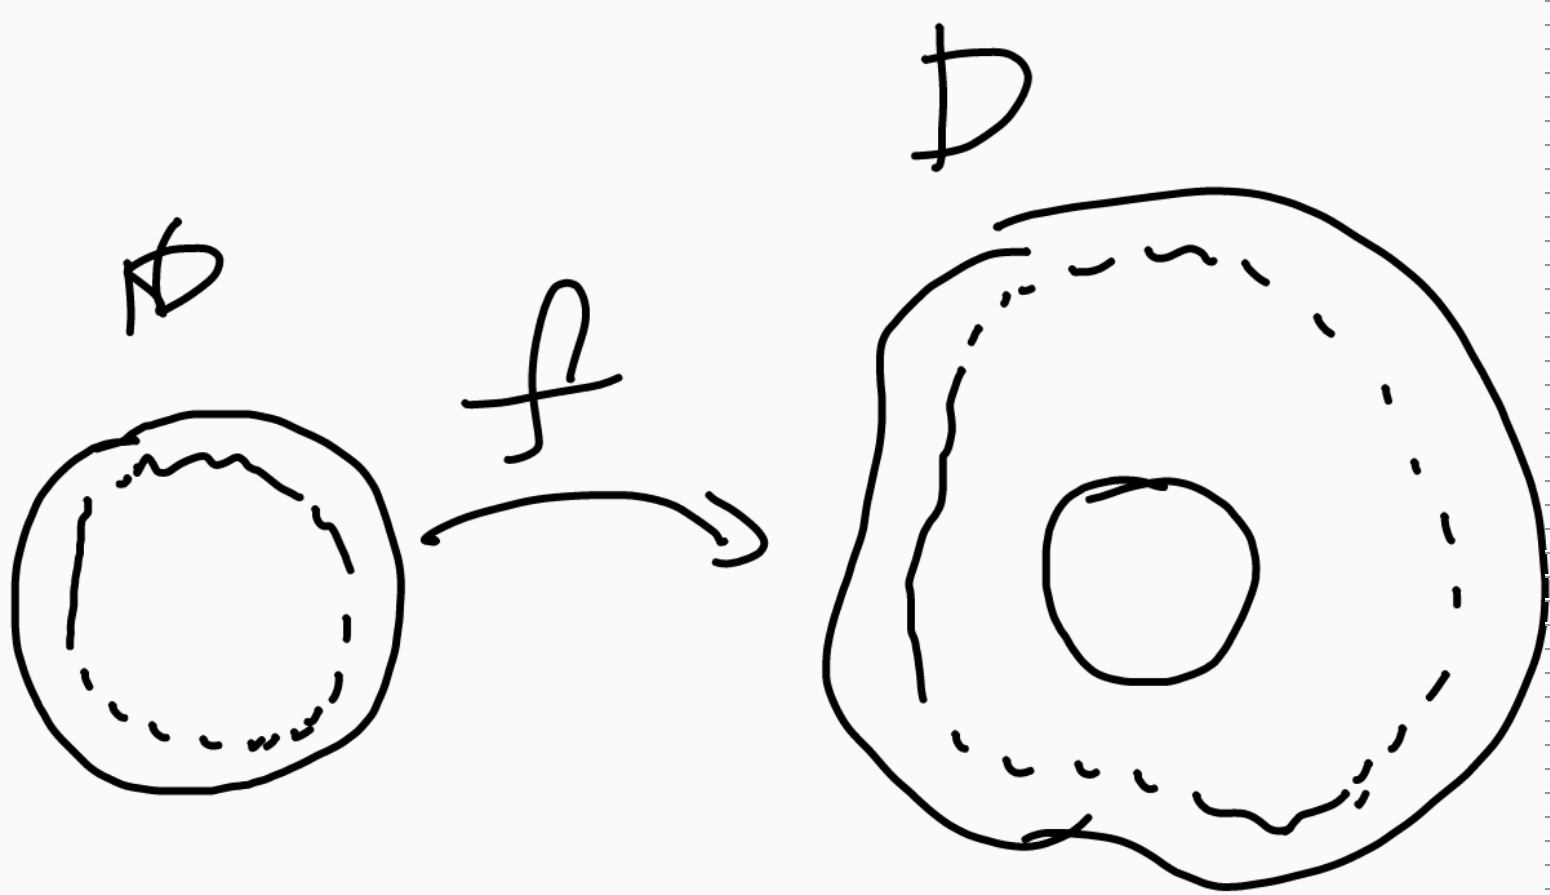
\includegraphics[scale =0.15]{3}
\end{center}
\end{figure}
\s

If $f\in U$, since $f(0) =0$, $f'(0)=1$, we have $f(z) = \sum_{n=0}^{\infty} a_n z^n = z+ \sum_{n=2}^{\infty} a_n z^n$.
\s

\propnum{1} If $f\in U$, then $|a_2|\leq 2$.
\s

This is related to Bieberbach conjecture : $|a_n|\leq n$ for all $n$. This is a famous complex analysis conjecture made in 1916. Loewner developed \emph{Loewner flows} while working on it. The conjecture was proved by de Branges in 1985.
\s

We will first prove the theorem assuming the propostion.

\begin{proof}
\textbf{proof of Koebe-1/4)} Suppose $f: \mathbb{D} \rightarrow D$ with $f\in U$. Fix $z_0 \not\in D$. The goal is to show that $|z_0| \geq 1/4$.

\quad Set $\tilde{f}(z) = \frac{z_0f(z)}{z_0- f(z)}$. Since $f\in U$, we have that
\begin{align*}
\tilde{f}(0) = \frac{z_0 f(0)}{z_0 - f(0)}=0, \quad \tilde{f}'(0)= \frac{z_0^2 f'(0)}{z_0^2} =1
\end{align*}
Moreover, $\tilde{f}$ is a conformal transformation as it is a composition of conformal transformations. Hence, we have $\tilde{f} \in U$.

\quad Write $f(z) = z + \sum_{n=2}^{\infty} a_n z^n$, then $\tilde{f}(z) = z+ (a_2 + \frac{1}{z_0})z^2 + \cdots$. By the proposition, we have $|a_2|\leq 2$ and $|a_2 + \frac{1}{z_0}|\leq 2$. So we have that
\begin{align*}
2\geq \Big|a_2 + \frac{1}{z_0}\Big| \geq \Big| \frac{1}{z_0} \Big| - |a_2| \geq \Big| \frac{1}{z_0} \Big| -2 
\end{align*}
Re-arranging, $\Big| \frac{1}{z_0}\Big| \leq 4$ and therfore $|z_0| \geq 1/4$. This gives the theorem for the case $r=1$.

\quad For general values of $r\in (0,1]$, the theorem follows by replacing $f$ with $f(rz)/r$.

\eop
\end{proof}

This theorem is useful in SLE, becuase it allows bound the derivative just using the geometry of the domain and the image. Conversely, one can bound the domain or the image just using the information of the derivative - often, dealing with derivative is much natural then dealing with the domain and the image. The following corollary captures this feature of the theorem very well.
\s

\corr Suppose $D, \tilde{D} \subset \mathbb{C}$ are domains, $z\in D$, $\tilde{z} \in \tilde{D}$, $f: D\rightarrow \tilde{D}$ is a conformal transformaiton with $f(z) = \tilde{z}$. Then :
\begin{align*}
\frac{\tilde{d}}{4d} \leq |f'(z)| \leq \frac{4\tilde{d}}{d}
\end{align*}
where $d= \text{dist}(z, \pa D)$ and $\tilde{d} = \text{dist}(f(z), \pa f(D))$.
\begin{proof}
\pf By translation, can assume that $z=\tilde{z} =0$. Let $\tilde{f}(w) = \frac{f(wd)}{f'(0)d}$. Then $\tilde{f}\in U$. So \emph{Koebe-1/4 theorem} gives $B(0, r/4) \subset f(r\mathbb{D})$ for all $r\in [0,1]$.

\begin{figure}[h]
\begin{center}
    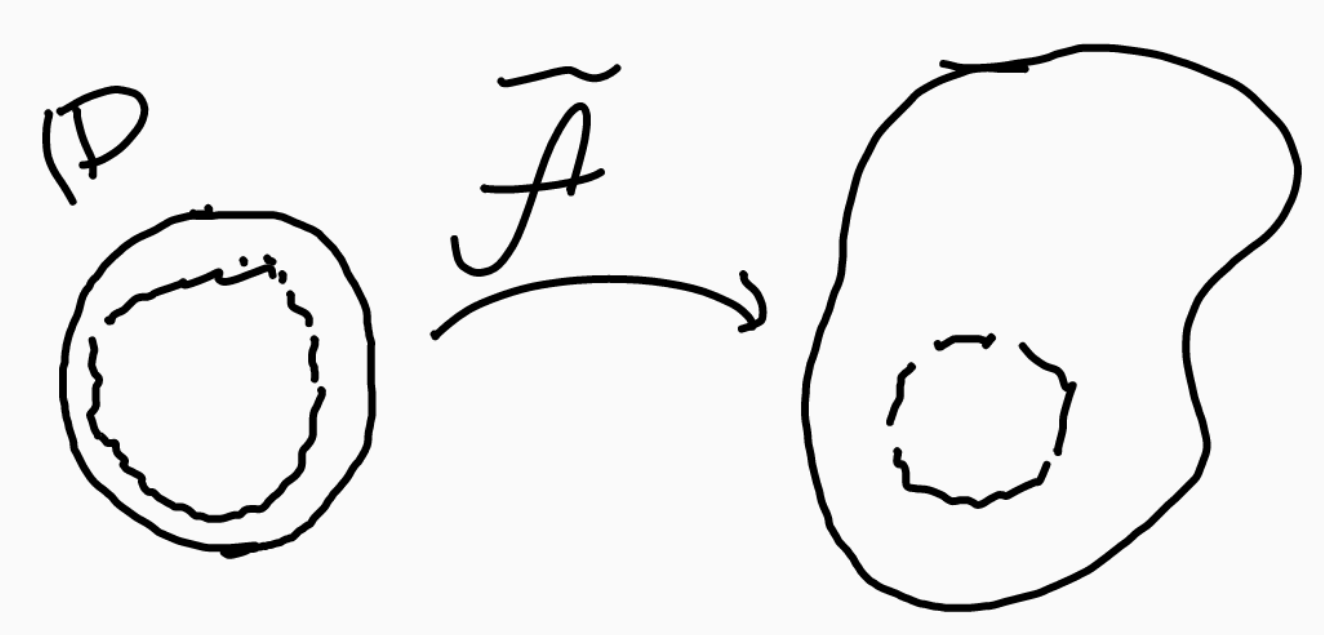
\includegraphics[scale =0.15]{4}
    \caption{in proof of corollary}
\end{center}
\end{figure}

For all $\epsilon>0$, there eixsts $\delta >0$ so that $\forall w\in \mathbb{D} \backslash (1-\delta) \mathbb{D}$ so that
\begin{align*}
\frac{\tilde{d}}{d|f'(0)|} \geq \Big| \frac{f(wd)}{f'(0)d}\Big| = |\tilde{f}(w)| \geq \frac{1}{4} - \epsilon
\end{align*}
By re-arranging, get $\tilde{d} \geq (\frac{1}{4} - \epsilon)d|f'(0)|$. Send $\epsilon \rightarrow 0$, then we obtain the upper bound.
\s

\quad To obtain the lower bound, use the same arguement with $f^{-1}$ in place of $f$ and not that $|(f^{-1})'(f(z))| = |f'(z)|^{-1}$.

\eop
\end{proof}
\s

Now we are just left to prove the propostion. However, the proposition is more trickier to prove than it looks. The proposition is proved using a series of methodology called \emph{area theorm}. The next propostion is the first version of \emph{area theorem}.
\s

\propnum{2} If $f\in U$, then $\text{area}(f(\mathbb{D})) = \pi \sum_{n=1}^{\infty} n|a_n|^2$.
\begin{proof}
\pf Fix $r\in (0,1)$, let $\gamma(0) = f(re^{i\theta})$, $\theta \in [0, 2\pi]$. Then
\begin{align*}
\frac{1}{2i} \int_{\gamma} \bar{z} dz &= \frac{1}{2i} \int_{\gamma} (x- iy) (dx + idy) \\
&= \frac{1}{2i} \int_{\gamma} \Big[ (x-iy)dx +(ix+y)dy\Big] \\
&= \frac{1}{2i} \int_{f(r\mathbb{D})} 2i dxdy = \text{area}(f(r\mathbb{D})) \quad \emph{[Green's formula]}
\end{align*}
On the other hand,
\begin{align*}
\frac{1}{2i} \int_{\gamma} \bar{z} dz &= \frac{1}{2i}\int_0^{2\pi} \overline{f(re^{i\theta})} f'(re^{i\theta}) ir e^{i\theta} d\theta \\
& = \frac{1}{2i} \int_0^{2\pi} \sum_{n=1}^{\infty}\bar{a}_n r^n e^{-i\theta n} \sum_{n=1}^{\infty} a_n n r^{n-1} e^{i\theta (n-1)} \cdot ire^{i\theta} d\theta\\
& = \pi \sum_{n=0}^{\infty} r^{2n} |a_n|^2 \cdot n
\end{align*}
Send $r\rightarrow 1$, then we are done.

\eop
\end{proof}
\s

\defi Say that $K\subset \mathbb{C}$ compact is a \textbf{compact hull} if $\mathbb{C}\backslash K$ is connected and $K$ consists of more than a single point. Let $\mathcal{H} = \{$compact hulls$\}$. 

\quad If $K\in \mathcal{H}$, \emph{Riemann mapping theorem} implies that there exists a unique conformal transformation $f: \mathbb{C} \backslash \bar{\mathbb{D}} \rightarrow \mathbb{C} \backslash K$ which fixes $\infty$ and has positive derivative at $\infty$, \textit{i.e.} $\lim_{z\rightarrow \infty} f(z)/z >0$.

\begin{figure}[h]
\begin{center}
    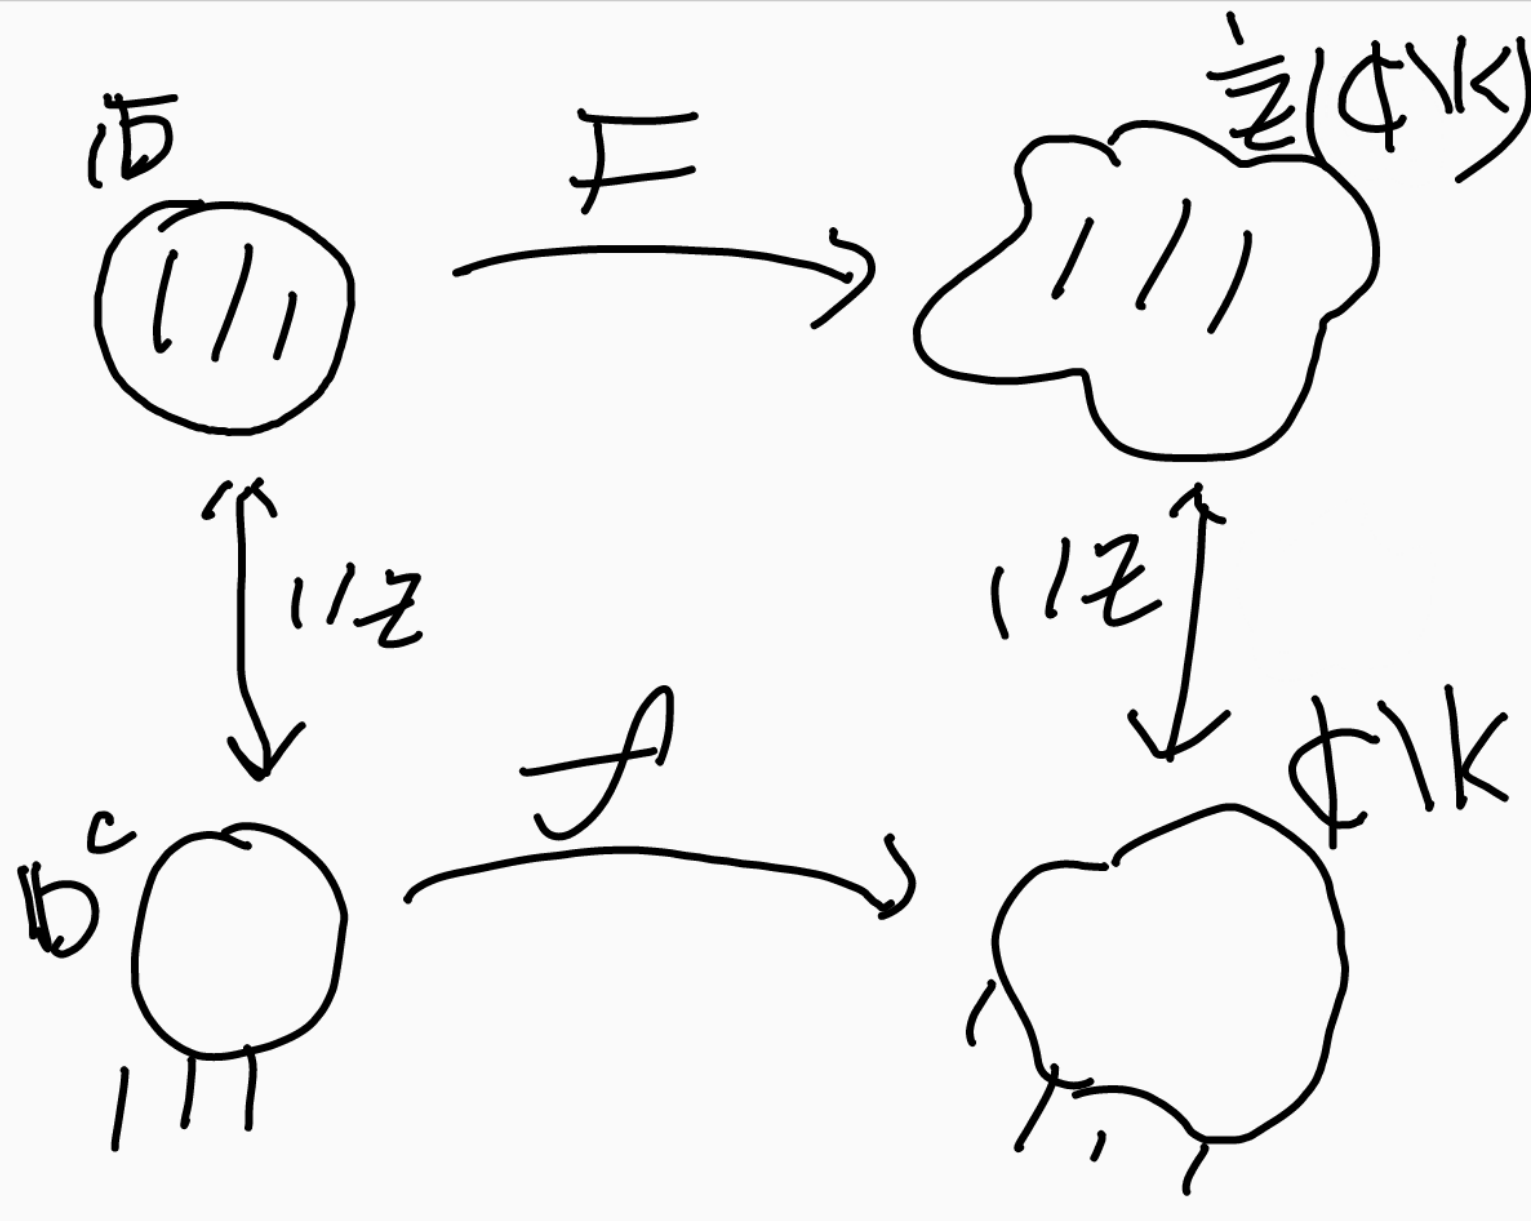
\includegraphics[scale =0.15]{5}
\end{center}
\end{figure}
\s

If $F$ is the unique conformal transformation $\mathbb{D} \rightarrow \frac{1}{z} (\mathbb{C}\backslash K)$ (the map $z\mapsto 1/z$ applied to $\mathbb{D} \backslash K$) with $F(0) =0, F'(0)>0$, then
\begin{align*}
f(z) = \frac{1}{F(1/z)}, \quad f(z)/z = \frac{1}{zF(1/z)} \xrightarrow{z\rightarrow \infty} \frac{1}{F'(0)}
\end{align*}
\s

The following is an another version of the \emph{area theorem}.
\s

\propnum{3} Suppose $K \in \mathcal{H}$ and $f(z) = z+ b_0 + \sum_{n=1}^{\infty}\frac{b_n}{z^n}$ be such that $f(\mathbb{D})=K$. Then 
\begin{align*}
\text{area}(K) = \pi \Big[ 1- \sum_{n=1}^{\infty} |b_n|^2 n\Big]
\end{align*} 
In particular, $\sum_{i=1}^{\infty} n|b_n|^2 \leq 1$.
\begin{proof}
\pf Fix $r>1$ and let $K_r = f(r\mathbb{D})$ and $\gamma = f(r \pa \mathbb{D})$. Then doing a bit of algebra,
\begin{align*}
\text{area}(K_r) = &\frac{1}{2i} \int_{\gamma}\bar{z} dz = \frac{1}{2i} \int_0^{2\pi} \overline{f(re^{i\theta})} f'(re^{i\theta}) \\
= &\Big[ r^2 - \sum_{n=1}^{\infty} n|b_n|^2 r^{-2n}\Big] \\
\xrightarrow{r\rightarrow 1}\,\, & \text{area}(K) = \pi\Big[ 1- \sum_{n=1}^{\infty} n|b_n|^2\Big]
\end{align*}
\eop
\end{proof}

Next time, we are going to finish proving $|a_2|\leq 2$ and start deriving Loewner's equation.
\s

\newday

(29th January, Tuesday)
\s

\textbf{Recap :} $U = \{\text{conformal transforamtions } f: \mathbb{D} \rightarrow D, f(0)=0, f'(0)=1 \}$.
\s

\lem If $f\in U$, then there exists $h\in U$ odd such that $h(z)^2 = f(z^2)$
\begin{p}
\pf Let
\begin{align*}
\tilde{f}(z) = \begin{cases}
f(z) /z \quad & z\neq 0 \\
f'(0) \quad & z=0 
\end{cases}
\end{align*}
Then $\tilde{f}$ is a non-zero holomorphic map on $\mathbb{D}$, so there exists a holomoprhic square-root of $\tilde{f}$, $g(z)^2 = \tilde{f}(z)$.  Set $h(z) = zg(z^2)$. Then $h$ is odd and
\begin{align*}
(h(z))^2 = z^2 (g(z^2))^2 = z^2 \cdot \tilde{f}(z^2) = f(z^2)
\end{align*}
Also, $h(0)=0$, $h'(0)=1$. We need to show $h$ is injective.
\begin{subproof}
: Suppose $h(z_1)= h(z_2)$, then $z_1 g(z_1^2) = z_2 g(z_2^2)$, so $z_1^2(g(z_1^2))^2 = z_2^2(g(z_2^2))^2$, and $f(z_1^2) = f(z_2^2)$, which implies $z_1^2 = z_2^2$ and so $g(z_1^2) = g(z_2^2)$. Recall $z_1g(z_1^2) = z_2 g(z_2^2)$, so we have $z_1 =z_2$.
\end{subproof}
Having this, we see that $h\in U$.

\eop
\end{p}
\s

\begin{p}
\textbf{proof of Proposition 1)} Suppose that $f\in U$. Suppose that $h\in U$ as in the lemma. since $h$ is odd, its series expansion only has odd powers of $z$ :
\begin{align*}
h(z) = z+ c_3 z^3 + c_5 z^5 + \cdots
\end{align*}
Also 
\begin{align*}
f(z^2) &= z^2 + a_2 z^4 + a_3 z^6 + \cdots = (h(z))^2 \\
&= (z+ c_3 z^3 + c_5 z^5 + \cdots)^2 = z^2 + 2c_3 z^4 +\cdots
\end{align*}
so $c_3 = a_2/2$. Let $g(z) = 1/h\Big(\frac{1}{z}\Big)$. Then
\begin{align*}
g(z) &= \frac{1}{z^{-1} + (a_2/2)z^{-3} + \cdots} = \frac{z}{1+(a_2/2)z^{-2} + \cdots}\\
&= z(1- \frac{a_2}{2}z^{-2} + \cdots) = z- \frac{a_2}{2}z^{-1} + \cdots
\end{align*}
so $|a_2/2|^2 \leq 1$ by \textbf{Proposition 3}. We conclude $|a_2| \leq 2$

\eop
\end{p}
\s

\subsection*{Half-plane capacity}

\defi Call $A\subset \mathbb{H}$ a \textbf{compact $\H$-hull} if $A = \bar{H} \cap \H$, $\H \backslash A$ are simply connected.

\quad Denote $\mathscr{Q} = \{$compact $\H$-hulls$\}$.
\s

We are going to be interested in (1) ``correct" notion of size of $A\in \mathscr{Q}$, (2) ``correct" conformal transformation $\H \backslash A \rightarrow \H$.
\s

\propnum{1} For each $A\in \mathscr{Q}$, there is a unique conformal transformation $g_A : \H \backslash A \rightarrow \H$ with $|g_A(z)-z| \rightarrow 0$ as $z\rightarrow \infty$ (that is, $g_A$ looks like the identity at $\infty$). 
\s

\propnum{2} \emph{(Schwarz reflection)} Let $D\subset \H$ be simply connected and $\phi : D \rightarrow \H$ be a conformal transformation which is bounded on bounded sets. Then $\phi$ extends by reflection to a conformal transformation on $D^* = D \cup \{\bar{z} : z\in D \} \cup \{ x\in \pa \H : D$ is a neighbourhood of $x$ in $\H\}$ by setting $\phi(\bar{z}) = \overline{\phi(z)}$.
\begin{p}
\pf Can find a proof in any complex analysis text. Also will be practicing a harmnoic function version of the theorem in the example sheet.
\end{p}
\s

\begin{p}
\textbf{proof of Propisition 1)} By the \emph{Riemann mapping theorem}, there exists a conformal transformation $g: \H \backslash A \rightarrow \H$. by post-composing $g$ with a conformal transformation $\H\rightarrow \H$, we may assume that $g$ fixes $\infty$. By Schwarz reflection, we can extend $g$ to a conformal transformation $\mathbb{C} \backslash ( \bar{A} \cup \{\bar{z} : z\in A\})$ by seetting $g(\bar{z}) = \overline{g(z)}$.

\quad By performing a series expansion for $1/(g(1/z))$, we see that
\begin{align*}
g(z) = b_{-1}z + b_0 + \sum_{n=1}^{\infty} b_n/z^n
\end{align*}
If $z\in \reals\backslash \bar{A}$, $z= \bar{z}$ and $g(z) = g(\bar{z}) = \overline{g(z)}$, so $g$ maps $\reals \backslash \bar{A}$ into $\reals$, so
\begin{align*}
b_{-1} z + b_0 + b_1 z^{-1} + \cdots = \bar{b_{-1}}z + \bar{b_0} + \bar{b_1} z^{-1} + \cdots
\end{align*}
Set $g_A(w) = \frac{g(w)-b_0}{b_{-1}}$, then we have $|g_A(z) - z| \rightarrow 0$ as $z\rightarrow \infty$.

\quad We are just left to show the uniqueness of such map. Suppose $\tilde{g}_A$ is another such conformal transformation. Then $\tilde{g}_A \circ g_A^{-1}$ is a conformal transforamtion $\H \rightarrow \H$. So by a standard propoerty of conformal map $\H \rightarrow \H$, we can find $a, b,c,d\in \reals$ with $ad-bc=1$ and
\begin{align*}
\tilde{g}_A \circ g_A^{-1} (z) = \frac{az+b}{cz+d}
\end{align*}
Since $|\tilde{g}_A \circ g_A^{-1} (z) -z| \rightarrow 0$ as $z\rightarrow \infty$, we should have $\tilde{g}_A \circ g_A^{-1} (z)=z$, and hence $\tilde{g}_A = g_A$.

\eop
\end{p}
\s

\defi If $A\in \mathscr{Q}$, the \textbf{half-plane capacity} of $A$ is
\begin{align*}
\text{hcap}(A) = \lim_{z\rightarrow \infty} z(g_A(z)-z)
\end{align*}
Equivalently, $g_A(z) = z + \frac{\text{hcap}(A)}{z} + \cdots$. $\text{hcap}$ is a notion of ``size" of $A$.

\quad We will prove several properties of $\text{hcap}$ that helps us interpret it as a ``size function".
\s

\textbf{Properties :} If $r>0$, $x\in \reals$, $A\in \mathscr{Q}$, then (i) $g_{rA} = rg_A(z/r)$, (ii) $g_{A+x} = g_A(z-x)+x$.

\quad Indeed, $rg_A(z/r)$ and $g_A(z-x) + x$ are the unique conformal transformations $\H \backslash (rA) \rightarrow \H$ and $\H \backslash (A+x) \rightarrow \H$, respectively, which look like the identity at $\infty$.

\quad As $rg_A(z/r) = z+ \frac{r^2 \text{hcap}(A)}{z} + \cdots$, so
\begin{i}
\item[(i)] $\text{hcap}(rA) = r^2 \text{hcap}(A)$, \emph{[scaling]}
\item[(ii)] $\text{hcap}(A+x) = \text{hcap}(A)$, \emph{[translation invariant]}
\end{i}
If $A, \tilde{A} \in \mathscr{A}$, $A\subset \tilde{A}$, then 
\begin{align*}
g_{\tilde{A}} = g_{g_A(\tilde{A} \backslash A)} \circ g_A
\end{align*}
as the RHS is the unique confromal transformation $\H \backslash \tilde{A} \rightarrow \H$ which looks like the identity at $\infty$.
\s

\newday

(31st January, Thursday)
\s

\textbf{Recap :} $\text{hcap} = \lim_{z\rightarrow \infty} z(g_A(z)-z)$, \textit{i.e.} $g_A(z) = z+ \frac{\text{hcap}(A)}{z} + \cdots$.
\s

If $A, \tilde{A} \in \mathscr{A}$, $A\subset \tilde{A}$, then 
\begin{align*}
g_{\tilde{A}} = g_{g_A(\tilde{A} \backslash A)} \circ g_A
\end{align*}
as the RHS is the unique confromal transformation $\H \backslash \tilde{A} \rightarrow \H$ which looks like the identity at $\infty$, so writing
\begin{align*}
& g_A(z) = z+ \frac{\text{hcap}(A)}{z} + \cdots \\
& g_{g_A(\tilde{A} \backslash A)} (z) = z + \frac{\text{hcap}(g_A(\tilde{A} \backslash A))}{z}+\cdots
\end{align*}
we have
\begin{align*}
g_{\tilde{A}}(z) = z+ \frac{\text{hcap}(\tilde{A})}{z} + \cdots = z+ \frac{\text{hcap}(A) + \text{hcap}(g_A(\tilde{A} \backslash A))}{z} + \cdots
\end{align*}
hence $\text{hcap}(\tilde{A}) = \text{hcap}(A) + \text{hcap}(g_A(\tilde{A}\backslash A))$. We will show in \textbf{Proposition 3} that $\text{hcap}\geq 0$, so this shows $\text{hcap}$ is monotone.
\s

\textbf{Examples :}
\begin{i}
\item[1.] $z\mapsto \sqrt{z^2 + 4t}$ is the unique conformal transformation $\H \backslash [0, 2i\sqrt{t}] \rightarrow \H$ with $|\sqrt{z^2 + 4t} - z| \rightarrow 0$ as $z\rightarrow \infty$. Then
\begin{align*}
\sqrt{z^2 + 4t} = z+ \frac{2t}{z} + \cdots
\end{align*}
so $\text{hcap}([0, 2i\sqrt{t}]) =2t$.
\item[2.] The map $z\mapsto z+ \frac{1}{z}$ maps $\H \backslash \bar{\D} \rightarrow \H$ with $|z+ \frac{1}{z}-z| \rightarrow 0$ as $z\rightarrow \infty$. So $\text{hcap}(\bar{\D} \cap \H) =1$.
\item[3.] If $A\in Q$ with $A\subset r(\bar{\D}\cap \H)$ for $r>0$, has
\begin{align*}
\text{hcap}(A) \leq \text{hcap}(r(\bar{\D}\cap \H)) = r^2 \text{hcap}(\D \cap \H) = r^2
\end{align*}
\end{i}
\s

\propnum{3} Suppose $A\in \mathscr{Q}$, $B$ a complex Brownian motion, and $\tau = \inf \{t\geq 0 : B_t \not\in \H \backslash A\}$. Then for all $z\in \H \backslash A$,
\begin{i}
\item[\textit{(i)}] $\text{Im} (z- g_A(z)) = \avg_z [\text{Im}(B_{\tau})]$.
\item[\textit{(ii)}] $\text{hcap}(A) = \lim_{y\rightarrow \infty} y \avg_{iy} [\text{Im}(B_{\tau})]$. In particular, $\text{hcap}(A) \geq 0$.
\item[\textit{(iii)}] $\text{hcap}(A) = \frac{2}{\pi} \int_{0}^{\pi} \avg_{e^{i\theta}} [\text{Im}(B_{\tau})] \sin \theta d\theta$, provided $A\subset \bar{\D}\cap \H$.
\end{i}
\begin{p}
\pf
\begin{i}
\item[\textit{(i)}] Note $\phi(z) = \text{Im}(z-g_A(z))$ is harmonic on $\H \backslash A$ as $z- g_A(z)$ is holomorphic. As $g_A(z) = z+ \frac{\text{hcap}(A)}{z} +\cdots$, it follows that $\phi(z)$ is bounded. Since $\text{Im}(g_A(z))=0$ when $z\in \pa (\H \backslash A)$, \textit{(i)} follows from the representatioin of harmonic functions using Brownian motion.
\item[\textit{(ii)}] 
\begin{align*}
\text{hcap}(A) &= \lim_{z\rightarrow \infty} z(g_A(z)-z) \\
&=\lim_{y\rightarrow \infty} iy (g_A(iy)-iy) \quad (\in \reals)\\
&= \lim_{y\rightarrow \infty} y \text{Im}(y - g_A(iy)) \quad (\text{took real part})\\
&=\lim_{y\rightarrow \infty} y\avg_{iy}  [\text{Im}(B_{\tau})] \quad (\text{by part } \textit{(i)})
\end{align*}
\item[\textit{(iii)}] See Example Sheets.
\end{i}
\end{p}
\s

\subsubsection*{Interlude}

\emph{Conformal invariance of Brownian motion :} up to a random time-change, the conformal image of a Brownian motion is a Brownian motion.
\s

\thm Let $D, \tilde{D} \subset \mathbb{C}$ be domains and $f: D\rightarrow \tilde{D}$ be a conformal transformation. Let $B, \tilde{B}$ be complex Brownian motions starting from $z\in D$, $\tilde{z} =f(z) \in \tilde{D}$, respectively. Let
\begin{align*}
\tau = \inf \{t\geq 0 : B_t \not\in D\}, \quad \tilde{\tau} = \inf \{t\geq 0: \tilde{B}_t\not\in \tilde{D} \}
\end{align*}
Let $\tau' = \int_0^{\tau} |f'(B_s)|^2 ds$ and 
\begin{align*}
& \sigma(t) = \inf\{ s\geq 0 : \int_0^s |f'(B_r)|^2 dr =t \} \\
& B_t' = f(B_{\sigma(t)})
\end{align*}
Then $(\tau', B_t' : t<\tau' ) \xeq (\tilde{\tau}, \tilde{B}_t : t< \tilde{\tau})$.
\begin{p}
\pf Use Stochastic Calculus, It\^{o}'s formula.

\eop
\end{p}

\s

Using the conformal invariance of Brownian motion, one can deduce that the first exit distribution of a Brownian motion is (see \emph{Example Sheet})


\begin{itemize}
\item from $\D$ starting from $z\in \D$ is $\frac{1}{2\pi} \Big[\frac{ 1-|z|^2 }{ |e^{i\theta} -z|^2 }\Big]$ at $e^{i\theta}$. (Recall, this is just the Poisson kernel)
\item from $\H$ starting at $z= x+ iy$ is $\frac{1}{\pi} \Big[ \frac{y}{(x-u)^2 + y^2} \Big]$ at $u\in \pa \H$.
\end{itemize}
\s

\prop Suppose that $A\in \mathscr{Q}$, $\text{rad}(A) = \sup \{ |z| : z\in A \}$. If $x> \text{rad}(A)$, $g_A(x) = \lim_{y\rightarrow \infty} \pi y \Big[ \frac{1}{2} - \prob_{iy} \big[ B_{\tau} \in (x, \infty) \big] \Big]$.

\quad If $x< -\text{rad}(A)$, $g_A(x) = \lim_{y\rightarrow \infty} \pi y \Big[ \frac{1}{2} - \prob_{iy} \big[ B_{\tau} \in (-\infty, x) \big] \Big]$.
\begin{p}


\pf Suppose $A= \phi$. Then
\begin{align*}
& \lim_{y\rightarrow \infty} \pi y \Big[ \frac{1}{2} - \prob_{iy} \big[ B_{\tau} \in (x, \infty) \big] \Big] = \lim_{y\rightarrow \infty} \pi y \prob_{iy} \big[ B_{\tau} \in [0,x] \big] \\
=& \lim_{y\rightarrow \infty} \pi y \int_0^x \frac{y}{\pi (u^2 + y^2)} du = \lim_{y\rightarrow \infty} \pi y \int_0^{x/y} \frac{1}{\pi(1+ u^2)} du =x = g_{\phi(x)}
\end{align*}
Now suppose $A\in \mathscr{Q}$ with $A \neq\phi$. Write $g_A(z) = u_A(z) + iv_A(z)$ and $\sigma  = \inf \{B_t \not\in \H \}$. By the conformal invariance of Brownian motion, 
\begin{align*}
\prob_{iy} [B_{\tau} \in (x,\infty)] &= \prob_{g_A(iy)} [B_{\sigma} \in (g_A(x) , \infty)] \\
&= \prob_{iv_A(iy)} [B_{\sigma} \in (g_A(x) - u_A(iy), \infty)] \quad (\text{translate by }-u_A(iy))
\end{align*}
As $y\rightarrow \infty$, $v_A(iy) / y \rightarrow 1$ and $yu_A(iy) \rightarrow 0$, as $g_A(iy) = u_A(iy) + i v_A(iy) = iy + \frac{\text{hcap}(A)}{iy} + \cdots$. By computing this probabilty in the limit $y\rightarrow \infty$ as before, the proposition follows.

\eop
\end{p}
\s

\newday

(5th February, Tuesday)
\s

\corr If $A\in \mathscr{Q}$, $\text{rad}(A)\leq 2$, then 
\begin{align*}
x\leq & g_A(x) \leq x + \frac{1}{x} \quad \text{if } x>1 \\
x+ \frac{1}{x} \leq & g_A(x) \leq x \quad \text{if } x<-1
\end{align*}
\begin{p}
\pf See Example Sheet \#1.
\end{p}
\s

\lem Let $p(z,e^{i\theta})$ be the exit distribution of a Brownian motion started from $z \in \H \backslash \D$ at point $e^{i, \theta}$ for $\theta \in [0, \pi ]$. Then it satisfies
\begin{align*}
p(z, e^{i\theta}) = \frac{2}{\pi} \frac{\text{Im}(z)}{|z|^2} \sin \theta (1+ O(1/|z|))
\end{align*}
\begin{p}
\pf See \emph{Example Sheet \#1}.
\end{p}

\s

\prop There exists $c>0$ so that for all $A\in \mathscr{Q}$, $|z| \geq \text{rad}(A)$, have that
\begin{align*}
\Big|g_A(z) - z - \frac{\text{hcap}(A)}{z}\Big| \leq c \cdot \frac{\text{rad}(A) \text{hcap}(A)}{|z|^2}
\end{align*}
\emph{[This tells us how good $z+ \text{hcap}(A)/z$ is as an estimate of $g_A(z)$. Also later, we will see that this is what we all need to prove Loewner's theorem.]}
\begin{p}
\pf By scaling, we can assume that $\text{rad}(A)=1$. Let $h(z) = z+ \frac{\text{hcap}(A)}{z} - g_A(z)$. Let 
\begin{align*}
v(z) = \text{Im}(h(z)) = \text{Im}(z- g_A(z)) - \frac{\text{hcap}(A)\text{Im}(z)}{|z|^2}
\end{align*}
Let $B$ be a complex Brownian motion and let $\sigma = \inf \{t\geq 0: B_t \not\in \H \backslash \overline{\mathbb{D}}\}$. For $\theta \in [0, \pi]$, let $p(z, e^{i\theta})$ be the density with respect to Lebesgue mesure of $B_{\sigma}$ at $e^{i\theta}$ of Brownian motion started at $z$. Then
\begin{align*}
\text{Im}(z- g_A(z)) = \int_0^{\pi} \avg_{e^{i\theta}}[\text{Im}(B_{\tau})] p(z, e^{i\theta})d\theta
\end{align*}
where $\tau = \inf \{t\geq 0 : B_t \not\in \H \backslash A\}$ by the strong Markov property of $B$.

Recall by the previous lemma, $p(z, e^{i\theta}) = \frac{2}{\pi} \frac{\text{Im}(z)}{|z|^2} \sin \theta (1+ O(1/|z|))$ and  by a previous result, $\text{hcap}(A) = \frac{2}{\pi} \int \avg_{e^{i\theta}}[\text{Im}(B_{\tau})] \sin \theta d\theta$. So
\begin{align*}
|v(z)| &= \Big|\text{Im}(z- g_A(z)) - \frac{\text{Im}(z)}{|z|^2} \text{hcap}(A)\Big| \\
&= \Big|\int_0^{\pi} \avg_{e^{i\theta}} [\text{Im}(B_{\tau})] p(z, e^{i\theta}) d\theta - \frac{2}{\pi}\int_0^{\pi} \avg_{e^{i\theta}}[\text{Im}(B_{\tau})] \sin \theta d\theta \cdot \frac{\text{Im}(z)}{|z|^2}\Big| \\
&\leq c\cdot \frac{\text{hcap}(A)\text{Im}(z)}{|z|^3} \quad \text{by previous lemma}
\end{align*}
where $c>0$ is a constant. Since $v$ is harmonic, by Example Sheet \#1, Problem \#8, can bound
\begin{align*}
|\pa_x v(z)| \leq c\frac{\text{hcap}(A)}{|z|^3}, \quad |\pa_y v(z)| \leq c\frac{\text{hcap}(A)}{|z|^3} \call{\star}
\end{align*}
Note that $h(iy) \rightarrow 0$ as $y\rightarrow \infty$, so 
\begin{align*}
|h(iy)| &= \big| \int_y^{\infty} h'(is)ds  \big| \leq \int_y^{\infty} |h'(is)|ds \\
&\leq \int_y^{\infty} c \frac{\text{hcap}(A)}{s^3} ds \quad \text{by } (\star) \text{ and the Cauchy-Riemann equation} \\
&\leq \tilde{c} \cdot \frac{\text{hcap}(A)}{y^2} \quad \text{for a constant } \tilde{c} >0
\end{align*}
\quad By a similar argument, except integrating along a semicircle of radius $r\geq 2$, have that
\begin{align*}
|h(re^{i\theta})| \leq & \int_{\pi/2}^{\theta} |h'(re^{i\theta})| rd\theta \\
\leq & c \cdot \frac{\text{hcap}(A)}{r^2} + |h(ir)| \\
\leq & c' \cdot \frac{\text{hcap}(A)}{r^2}
\end{align*}

\eop
\end{p}
\s

\subsubsection*{Chordal Loewner equation}

\thm \emph{(Beurling estimate)} There exists a constant $c>0$ so that the following is true. Let $B$ be a complex Brownian motion $A\subset \overline{\D}$, with $0\in A$, $A\cap \pa \overline{\D} \neq \phi$, connected. Then
\begin{align*}
\prob_z [ B([0, \tau]) \cap A = \phi] \leq c|z|^{1/2}, \quad z\in \D 
\end{align*}
where $\tau =\inf \{t\geq 0 : B_t \not\in \D \}$ and $B([0, \tau]) = \{B_t : t\in [0, \tau] \}$. \emph{[Note that the constant $c$ does not depend on the set $A$ - this makes this estimate useful.]}

\begin{p}
The worst case behavior is attined for $A = [0,1]$. To see this, consider a conformal map $\D \backslash [0,1] \rightarrow \H$ which fixes 0 behaves like the map $z\mapsto \sqrt{z}$ near 0. (needs a diagram)
\s

Theorem is quite tricky to prove, so will skip it here. However, it is not difficult to show that the theorem holds with $\frac{1}{2}$ replaced by some constant $\alpha>0$ (which is not obtained explicit, but does not depend on $A$).
\s

\textbf{Idea :} fix $r>0$, and let $C_r = B(0, r) \backslash \overline{B(0, r/2)}$. Complex Brownian motion starting from $-\frac{3}{4}ir$ has a positive chance $p_0$ of disconnecting 0 from $\infty$ before leaving $C_r$ (that is, going around the origin not leaving $C_r$). Moreover, $p_0$ does not depend on $r$. [can deduce using the first exit disribution of Brownian motion from a disk when started at its center is uniform.]

\quad Then partition the annulus $B(0, 1) \backslash B(0, |z|)$ in to annuli
\begin{align*}
C_k = B(0, \pa^k |z|) \backslash \overline{B(0, 2^{k-1}|z|)}
\end{align*}
for $1\leq k \leq \lceil \log_2 1/|z| \rceil$. For $B$ to make it to $\pa \D$ without hitting $A$, it must have been that it did not disconnect 0 from $\infty$ in the time interval between when it first hits $\pa B(0, \frac{3}{4} 2^{k-1} |z|)$ and when it subseqeuntly exits $C_k$. Therefore the probabiilty that $B$ does not hit $A$ is
\begin{align*}
\leq (1-p_0)^{\lceil \log_2 (1/|z|) \rceil} = |z|^{\alpha} \quad \text{for } \alpha = \alpha(p_0)
\end{align*}
\end{p}
\s

\newday

(7th February, Thursday)
\s

(Announcement : Class on February 12 (next Tuesday) to be mdae up a later point in the term)
\s

\textbf{Today :} We need one more estimate. Then prove Loewner's theorem, derive SLE. 
\s

\prop There exists a constant $C>0$ so that the following holds. Suppose $A, \tilde{A} \in \mathscr{Q}$ with $A\subset \tilde{A}$, $\tilde{A}\backslash A$ connected. Then
\begin{align*}
\text{diam}(g_A(\tilde{A}\backslash A))\leq C \begin{cases}
(dr)^{1/2} & \quad d\leq r \\
\text{rad}(\tilde{A}) & \quad d>r
\end{cases}
\end{align*}
where $d = \text{diam}(\tilde{A} \backslash A)$, $r =\sup \{\text{Im}(z) : z \in \tilde{A} \}$
\begin{p}
\pf By scaling, can assume that $r=1$.

\quad If $d>1$, the bound follows since : $|g_A(z)-z| \leq 3\text{rad}(A)$ (\emph{Example Sheet \#1}). So
\begin{align*}
\text{diam}(g_A(\tilde{A}\backslash A)) \leq \text{diam}(\tilde{A}) + 6 \text{rad}(A) \leq 8 \text{rad}(\tilde{A})
\end{align*}

\quad Next assume that $d<1$. Let $B$ be a complex Brownian motion starting from $iy$, $y\geq 2$. Let $U =B(z,d)$ be chosen so that $U \supset \tilde{A} \backslash A$. Let $\tau = \inf \{t\geq 0: B_t \not\in \H \backslash A \}$. For $B[0, \tau]$ to hit $U$, it must 
\begin{i}
\item[(1)] Reach $B(z,1)$ before leaving $\H \backslash A$. This happens with probability $\leq c/y$, $c>0$ constant,
\item[(2)] Given (1) has happend, must reach $U$ before leaving $\H\backslash A$. Beurling estimte says that this happens with probability $\leq cd^{1/2}$, $c>0$ constant.
\end{i}
Therefore, $\limsup_{y\rightarrow \infty} y \prob_{iy} [B[0, \tau] \cap U \neq \phi] \leq cd^{1/2}$. By the conformal invariance of Brownian motion, with $\sigma = \inf\{t\geq 0 : B_t \not\in \H \}$, has
\begin{align*}
\limsup_{y\rightarrow \infty} y\prob_{iy} [B[0, \sigma] \cap g_A(\tilde{A}\backslash A) \neq \phi]\leq cd^{1/2}
\end{align*}
Since $g_A(\tilde{A} \backslash A)$ is connected, by Example Sheet \#1, has $\text{diam}(g_A(\tilde{A} \backslash A))\leq cd^{1/2}$.

\eop
\end{p}
\s

\defi Now suppose $(A_t)$ is a family of compact $\H$-hulls with $A_0 = \phi$. Say that $(A_t)$ is
\begin{i}
\item[(i)] \textbf{non-decreasing} if $s\leq t$ implies $A_s\subset A_t$.
\item[(ii)] \textbf{locally growing} if $\forall T>0$, $\epsilon >0$, $\exists \delta >0$ so that $0\leq s\leq t \leq s+\delta T$ implies $\text{diam}(g_s (A_t \backslash A_s))\leq \epsilon$.
\item[(iii)] \textbf{parameterized by capacity} if $\text{hcap}(A_t)=2t$ for all $t\geq 0$.
\end{i}
Let 
\begin{align*}
&\mathscr{A} = \{\text{families of compact } \H\text{-hulls satisfying (i),(ii),(iii)} \} \\
&\mathscr{A}_T = \{\text{families of compact } \H\text{-hulls satisfying (i),(ii),(iii) defined on }[0,T] \}
\end{align*}
Surely, $\mathscr{A} = \mathscr{A}_{\infty}$.
\s

\textbf{Example :} Proposition implies that if $\gamma$ is a simple curve in $\H$ starting from 0, then $A_{t} = \gamma [0,t]$ gives a family in $\mathscr{A}$. Also in Example sheet \#1, Problem \#11, will see that the can be parameterized by capacity.
\s

\prop Suppose $(A_t) \in \mathscr{A}$, $g_t = g_{A_t}$. Then there exists $U :[0, \infty) \rightarrow \reals$ continuous so that
\begin{align*}
\pa_t g_t(z) = \frac{2}{g_t(z)- U_t}, \quad g_0(z)=z
\end{align*}
\begin{p}
\pf First note that $\bigcap_{s>t} \overline{g_t(A_s)}$ consists of a single point since $(A_t)$ is locally growing (hence $\overline{g_t(A_s)}$ are bounded, and therefore forms a nested family of compact sets). Set $U_t$ to be this point. It is easy to see that $U_t$ is continuous since $(A_t)$ is locally growing. 

\quad Recall if $B\in \mathscr{Q}$, then $g_B(z) = z+ \frac{\text{hcap}(B)}{z} + O \Big( \frac{\text{hcap}(B)\text{rad}(A)}{|z|^2} \Big)$ and that if $x\in \reals$, then $g_{B+x}(z)-x = g_B(z-x)$. So
\begin{align*}
g_B(z) = g_{B+x}(z+x)-x = z+ \frac{\text{hcap}(B)}{z+x}+ \text{hcap}(B)\text{rad}(B+x) O \Big(\frac{1}{|z+x|^2}\Big) \call{\star}
\end{align*}
Fix $\epsilon >0$. For $0\leq s\leq t$, let $g_{s,t} = g_t \circ g_s^{-1}$. Note that since $(A_t)$ is parametrized by capacity and $\text{hcap}(A_{t+ \epsilon}) = \text{hcap}(A_t) + \text{hcap}(g_t(A_{t+\epsilon} \backslash A_t ))$, we have $\text{hcap}(A_{t+\epsilon} \backslash A_t )) = 2\epsilon$. Apply $(\star)$ with $B = g_t(A_{t+ \epsilon}\backslash A_t)$, $x= -U_t$, and use that $\text{rad}(B-U_t) \leq \text{diam}(B)$ to see that
\begin{align*}
g_{t, t+\epsilon}(z) = z+ \frac{2\epsilon}{z-U_t} + 2\epsilon \cdot \text{diam}(B) O\Big(\frac{1}{|z-U_t|^2}\Big)
\end{align*}
so
\begin{align*}
g_{t+\epsilon}(z) - g_t(z) &= (g_{t, t+\epsilon} - id) \circ g_t (z) \\
& = \frac{2\epsilon}{g_t(z)- U_t} + 2\epsilon \text{diam}(g_t(A_{t+\epsilon}\backslash A_t)) O\Big(\frac{1}{|g_t(z)- U_t|^2} \Big)
\end{align*}
Divide both sides by $\epsilon$, send $\epsilon \rightarrow 0$, get that $\pa_t g_t(z) = \frac{2}{g_t(z)- U_t}$.

\eop
\end{p}
\s

Conversely, if $U: [0, \infty )\rightarrow \reals$ is continuous, then we can let $(g_t)_{t\geq 0}$ to solve
\begin{align*}
\pa_t g_t(z) = \frac{2}{g_t(z) - U_t}, \quad g_0(z)=z
\end{align*}
Then $A_t = \H \backslash \text{Image}(g_t)$ is a family in $\mathscr{A}$. [\emph{Example Sheet \#1}]. Here, $U$ is called the \textbf{``Loewner driving function"}. (However, the corresponding $g$ is not always a curve)
\s

\subsubsection*{Derivation of SLE}

\defi Suppose that $(A_t)$ is a random family in $\mathscr{A}$ encoded by $U$. Let $\FF_t = \sigma(U_s : s\leq t)$. We say that $(A_t)$ satisfies the \textbf{conformal Markov property} if
\begin{i}
\item[(i)] \textbf{(``Markov")} Given $\FF_t$, $(g_t(A_{t+s}\backslash A_t) - U_t)_{s\geq 0} \xeq (A_s)_{s\geq 0}$.
\item[(ii)] \textbf{(``Conformal")} Is scale invariant in that $(rA_{t/r^2})_{t\geq 0} \xeq (A_t)$ for all $r>0$. \emph{[called ``conformal" since the only conformal transformations $\H\rightarrow \H$ which fix $0, \infty$ are rescaling.]} 
\end{i}
\s

\thm \emph{(Schramm)} If $(A_t)$ satisfies the \emph{conformal Markov property}, then there exists $\kappa >0$ so that $U = \sqrt{\kappa} B$, where $B$ is a standard Brownian motion.
\s

\defi The family $(g_t)$ with $U =\sqrt{\kappa} B$ is called $\text{SLE}_{\kappa}$.

Later : We will see properties of $g_t$ depending on the values of $\kappa$.
\s

\newday

(14th February, Thursday)
\s

(example class 1 at Feb 21 in MR15, 2pm or 4pm. Submit solutions to question 9 and 10 to pigeon hole of jason miller, unitl 5pm Feb 19)
\s

\thm \emph{(Schramm)} If $(A_t)$ satisfies the \emph{conformal Markov property}, then there exists $\kappa >0$ so that $U = \sqrt{\kappa} B$, where $B$ is a standard Brownian motion.
\begin{p}
\pf Condition (i) of conformal Markov property is
\begin{align*}
& (U_{t+s} -U_t)_{s\geq 0} \xeq (U_s)_{s\geq 0} \quad \text{given } \FF_t \\
\Leftrightarrow \quad & (U_t) \text{ has stationary independent incremetns} \\
\Rightarrow \quad &\exists \kappa \geq 0, a\in \reals \text{ so that } U_t = \sqrt{\kappa} B_t + at \text{ where B is a standard BM}
\end{align*}
Condition (ii) of conformal Markov property is saying that 
\begin{align*}
(rA_{t/r^2}) \xeq (A_t) \quad \Leftrightarrow \quad (rU_{t/r^2}) \xeq (U_t) \quad (U \text{ satisfies Brownian scaling)}
\end{align*}
so
\begin{align*}
\sqrt{\kappa} \tilde{B}_t + at \xeq rU_{t/r^2} =  \sqrt{\kappa} rB_{t/r^2} + ar\cdot \frac{t}{r^2} \xeq  \sqrt{\kappa} \tilde{B}_t + \frac{a}{r}{t} \quad (\tilde{B} \text{ a standard BM}) 
\end{align*}
where the first equality makes use of property (ii). So $a=0$.

\eop
\end{p}
\s

For $\kappa\geq 0$, $SLE_{\kappa}$ is the random family of hulls encoded by $U_t = \sqrt{\kappa} B_t$, $B$ a standard BM. Also, $SLE_{0}$ has $U(t) = 2\sqrt{t} i$.
\s

\textbf{Remarks :}
\begin{i}
\item[(1)] $SLE_{\kappa}$ is generated by a continuous curves. This measn that for all $t\geq 0$, $\H \backslash A_t=\text{unbounded compnent of } \H\backslash \gamma[0,t]$. This was proves by Rohde-Scharamm, and we will take this as an ssumption in this course.
\item[(2)] Behaviour of $SLE_{\kappa}$ depend strongly on $\kappa$. We will show that $SLE_{\kappa}$ is
\begin{i}
\item[(i)] \emph{Simple} if $\kappa \in (0,4]$.
\item[(ii)] \emph{Self-intersecting} if $\kappa \in (4,8)$ - In this case, $A_t$ corresponds to $\gamma[0,t]$ with holes filled in.
\item[(iii)] \emph{Space-filling} if $\kappa \geq 8$.
\end{i}
\begin{figure}[h]
\begin{center}
    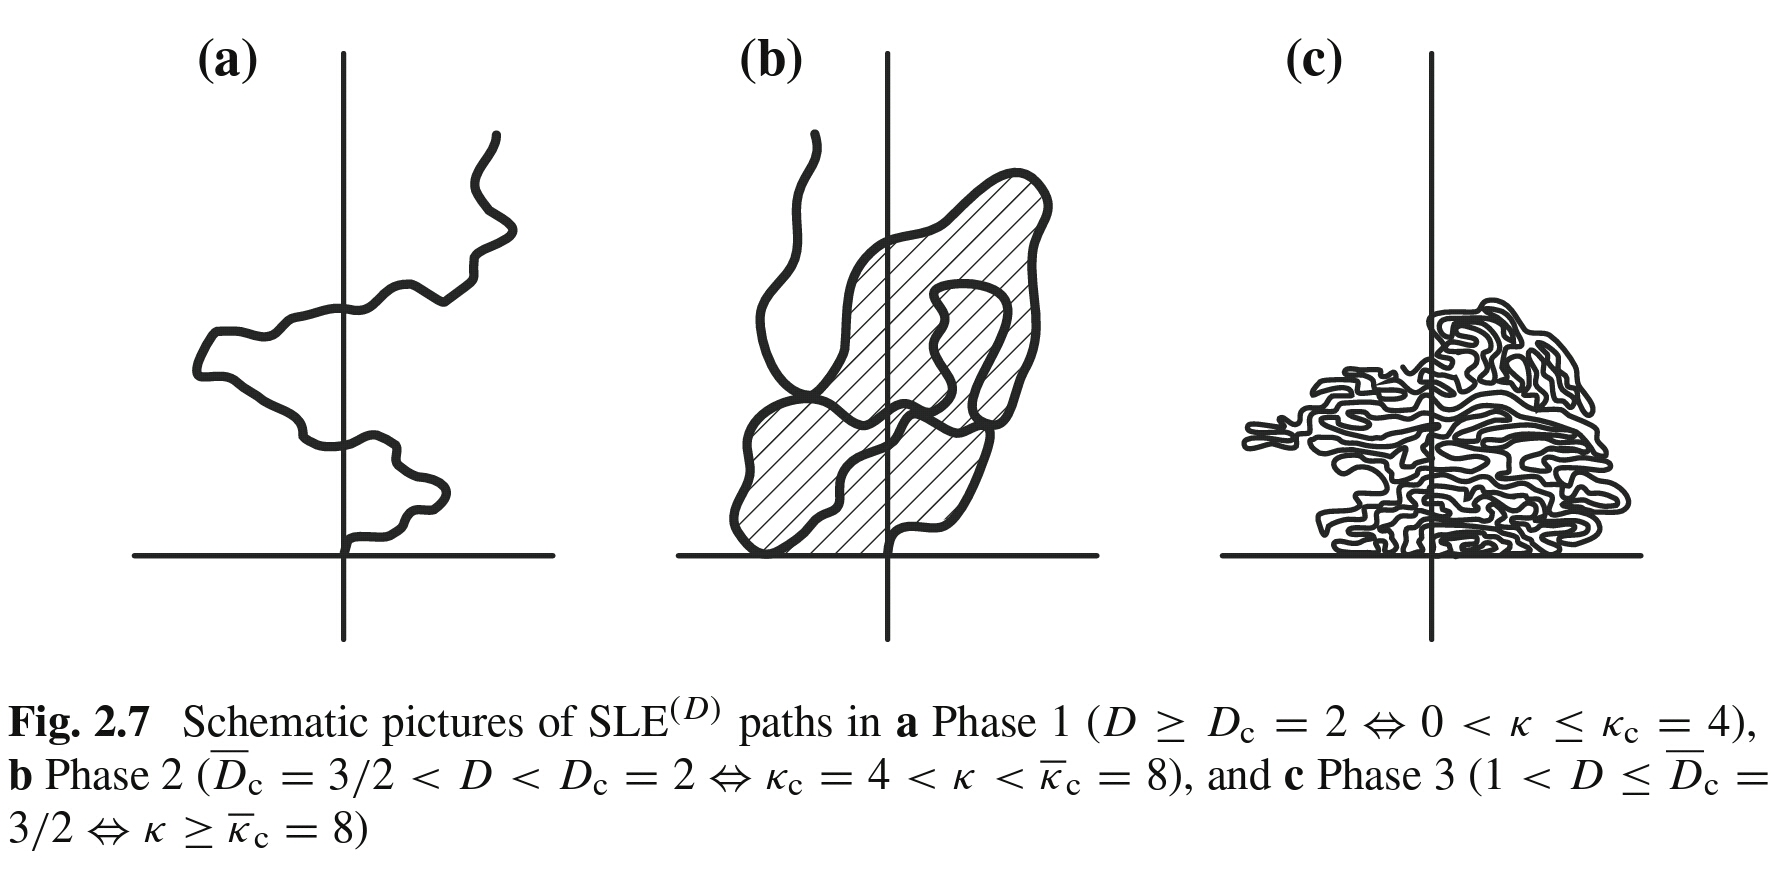
\includegraphics[scale =0.15]{6}
    \caption{reference : M. Katori, ``Bessel Processes, Schramm-Loewner Evolution and the Dyson Model" (2015)}
\end{center}
\end{figure}
\item[(3)] $SLE_{\kappa}$ is singled out by the conformal Markov property. This comes from conjecture from the physics literature, about scaling limits of discrte models, \textit{e.g. percolation}.
\item[(4)] Important tool : Stochastic calculus.
\end{i}
\s

\subsubsection*{Stochastic Calculus Review}

(Yippi!!!)

Basic object of study is continuous semi-martingale,
\begin{align*}
X_t = M_t + A_t
\end{align*}
where $M$ is a continuous local martingale and $A$ a bounded variation process.
\s

\textbf{Important concepts :}
\begin{i}
\item[(1)] Stochastic integral
\item[(2)] Quadratic variation
\item[(3)] It\^o formula
\item[(4)] Levy characterization.
\item[(5)] SDE's
\end{i} 
\s

\textbf{General Setting :} One has probability space $(\Omega, \FF, \prob)$ with a filtration $(\FF_t)$ satisfying the \textbf{``usual conditions"}.
\begin{i}
\item[(i)] $\FF_0$ contains all $\prob$-null sets.
\item[(ii)] $\FF_t$ is right-continuous, \textit{i.e.} $\FF_t =\bigcap_{s>t} \FF_s$.
\end{i}
\s

\textbf{Stochastic Integral :} $X_t = M_t + A_t$ continuous semi-martingale, $H_t$ a prvisible process. Set 
\begin{align*}
\int_0^t H_s dX_s = \int_0^t X_s dM + \int_0^t H_s dA_s
\end{align*}
where the first integral is It\^o integral for continuous local martingales and the second one is Lebesgue-Stieljes integral continuous with bounded variation. We have defined and constructed the stochastic integral in the spirit of the Riemann integral - it is not a measure. It is the extra cancellation in the definition of the It\^o intgral which makes it converge.
\s

\textbf{Quadratic variation} of a continous local martingale $M_t$ is
\begin{align*}
[M]_t = \lim_{n\rightarrow \infty} \sum_{k=1}^{\lceil 2^nt \rceil -1} (M_{(k+1)2^{-n}} -M_{(k)2^{-n}})^2
\end{align*}
This is characterized by the property that it is the unique continuous process of bounded variation so that $M^2 - [M]$ is a continuous local martingale. 

\quad Quadratic variation of a continuous finite variation process vanishes. So
\begin{align*}
[X]_t = [M+A]_t = [M]_t
\end{align*}
Also,
\begin{align*}
\Big[ \int_0^{\cdot} H_s dM_s \Big]_t = \int_0^t H_s^2 d[M]_s
\end{align*}
which is just a Lebesgue-Stieltjes integral. 
\s

\textbf{It\^o's formula :} This is just a stochastic analogue of the \emph{Fundamental Theorem of Calculus}. If $f\in C^2$, then
\begin{align*}
f(t) = f(0) + \sum_{k=1}^n (f(t_k)- f(t_{k-1}))
\end{align*}
where $0=t_0 < \cdots < t_n =t$ is a partition of $[0,t]$. By Taylor's formula,
\begin{align*}
f(t) = & f(0) + \sum_{k=1}^n \big(f'(t_{k-1})(t_{k}- t_{k-1}) + o(t_k -t_{k-1})\big) \\
\rightarrow & f(0) + \int_0^t f'(s) ds \quad \text{as } \max |t_k -t_{k-1}| \rightarrow 0
\end{align*}
In a similar context, suppose $B$ is a Brownian motion with $B_0 =0$ and make Taylor expension with point $B_t$ :
\begin{align*}
f(B_t) = & f(B_0) + \sum_{k=1}^n \big( f'(B_{t_{k-1}}))(B_{t_k} -B_{t_{k-1}}) + \frac{1}{2} f''(B_{t_{k-1}})(B_{t_k}-B_{t_{k-1}})^2 + o((B_{t_k} -B_{t_{k-1}})^2 )\big)  \\
\rightarrow & f(0) + \int_0^t f'(B_s) dB_s + \frac{1}{2} \int_0^t f''(B_s) ds
\end{align*}
since the summation over the quadratic terms is not negligible anymore in this setting.

\quad We can make the general version accrodingly. If $X_t = M_t + A_t$ is a contiuous semi-martingale, with $f\in C^{1,2}(\reals_{+}\times \reals)$ then
\begin{align*}
& f(t, X_t) = f(0, X_0) + \int_0^t \pa_s f(s, X_s) ds + \int_0^t \pa_x f(s, X_s) dX_s + \frac{1}{2} \int_0^t \pa_x^2 f(s, X_s) d[M]_s \\
& = f(0, X_0) + \Big[ \int_0^t \pa_s f(s, X_s)ds + \int_0^t \pa_x f(s, X_s)dA_s + \frac{1}{2} \int_0^t \pa_x^2 f(s, X_s) d[M]_s\Big] + \int_{0}^t \pa_x f(s, X_s) dMS
\end{align*}
\s

\textbf{Example :} For a standard Brownian motion $B_t$, $B_t^2 = B_0^2 + \int_0^t 2 B_s dB_s +t$, so $B_t^2 -t = 2\int_0^t B_s dB_s$ is a martingale.
\s

\textbf{L\'evy Characterization :} If $M$ is a continous local martingale, then $M$ is a standard Brownian motion \emph{iff} $[M]_t =t$.
\begin{p}
\pf Use It\^o's formula with $e^{i\theta M_t + \frac{1}{2}\theta^2 [M]_t}$ - this is called an \emph{exponential martingale.} So one can calculate the characteristic function of $M_t$ from this.

\eop
\end{p}
\s

\textbf{Stochastic differential equations :} $(\Omega, \FF, \prob)$, $(\FF_t)$ be satisfying the usual conditions. Suppose $B$ is a standard Brownian motion adapted to $(\FF_t)$. For function $b, \sigma$, we say a process $(X_t)$ solves the SDE
\begin{align*}
dX_t = b(X_t) dt + \sigma(X_t) dB_t
\end{align*}
if and only if
\begin{align*}
X_t =X_0 + \int_0^t b(X_s)ds + \int_0^t \sigma(X_s) dB_s \quad \forall t\geq 0
\end{align*}
One can prove existence/uniqueness when $b$, $\sigma$ are Lipschitz functions. \emph{[This will be done in the Stochastic Calculus course.]}
\s

\newday

(19th Tuesday)
\s

(Example class \#1 at 1:30 Thursday 21st MR15 or 4:00 pm Friday 22nd MR5)
\s

\textbf{Goal : Estblish phases of $\text{SLE}_{\kappa}$}.

\subsection*{Bessel Processes}

Suppose that $X = (B^1, \cdots, B^d)$ is a $d$-dimensional Brownian motion. Let $Z_t = \norms{X_t}{} = \big( (B_t^1)^2 + \cdots + (B_t^d)^2 \big)^{1/2}$. It\^o's formula implies
\begin{align*}
Z_t^2 =& (B_t^2) + \cdots + (B_t^d)^2 \\
=& Z_0^2 + 2\int_0^t B_s^1 dB_s^1 + \cdots + 2\int_0^t B_s^t dB_s^d + td
\end{align*}
Set $Y_t = \int_0^t \frac{B_s^1 dB_s^1 + \cdots + B_s^d dB_s^d}{Z_s}$, then
\begin{align*}
Z_t^2 = Z_0^2 + 2\int_0^t Z_s dY_s + td
\end{align*}
Note $[Y]_t =\int_0^t \frac{(B_s^1)^2 + \cdots + (B_s^d)^2}{Z_s^2}ds =t$ and also $Y_t$ is a continuous local martingale. Therefore, the \emph{L\'evy characterization} implies $Y_t$ is a standard Brownianm motion. So letting $\tilde{B}_t = Y_t$,
\begin{align*}
& Z_t^2 = Z_0^2 + 2\int_0^t Z_s d \tilde{B}_s + td \\ 
\Leftrightarrow \quad & dZ_t^2 = 2Z_s d\tilde{B}_s + dt \cdot d  
\end{align*}
This is referred as \textbf{squared Bessesl SDE with dimension d} and $Z_t^2$ is a \textbf{squared Bessel process with dimension $d$} and denoted $\text{BESQ}^d$.
\s

Apply It\^o's formula with $f(x) = \sqrt{x}$ and insert the expression for $d(Z_t^2)$ above to see that 
\begin{align*}
Z_t =& Z_0 + \frac{1}{2} \int_0^t Z_s^{-1} d(Z_s^2) - \frac{1}{8} \int_0^t Z_s^{-3} d[Z^2]_s  \\
=& Z_0 + \tilde{B}_t + \frac{d}{2} \int_0^t Z_s^{-1} ds - \frac{1}{2} \int_0^t Z_s^{-1} ds \\
=& Z_0 + \tilde{B}_t + \frac{d-1}{2}\int_0^t Z_s^{-1} ds \\
\Leftrightarrow \quad & dZ_t = \frac{d-1}{2} Z_t^{-1} dt + d\tilde{B}_t 
\end{align*}
This is called \textbf{Bessel SDE of dimension $d$} and $Z_t$ is a \textbf{Bessel process of dimension $d$} and denoted $\text{BES}^d$. For $d\in \mathbb{N}$, a $\text{BES}^d$ corresponds to the modulus of a $d$-dimensional Brownian motion. However, the $\text{BES}^d$ SDE has a solution for all $d\in \reals$, up until hitting 0.
\s

\textbf{$\heartsuit$ Claim :} If $d\in \reals$, $Z_t$ is a $\text{BES}^d$, then
\begin{i}
\item $d<2$ then $Z_t$ hits 0 almost surely.
\item $d\geq 2$ then $Z_t$ almost surely does not reach 0.
\end{i}
\emph{[If $d=2$, the Bessel process gets arbitrarily close to 0 infinitely often without hitting 0 as a 2-diemnsional Brownian motion does not hit 0, but gets arbitrarily close]}
\begin{p}
\pf Consider $Z_t^{2-d}$. By It\^o's formula and expression for $dZ_t$,
\begin{align*}
Z_t^{2-d} =& Z_0^{2-d} + \int_0^t (2-d) Z_t^{1-d} dZ_t + \frac{1}{2} \int_0^t (2-d)(1-d) Z_t^{-d} d[Z]_t \\
=& Z_0^{2-d} + \int_0^t (2-d) Z_t^{1-d} d\tilde{B}_t +\int_0^t \frac{(2-d)(d-1)}{2} Z_t^{-1} dt + \frac{1}{2} \int_0^t (2-d)(1-d) Z_t^{-1} dt \\
=& Z_0^{2-d} + \int_0^t (2-d) Z_t^{1-d} d\tilde{B}_t
\end{align*}
So $Z_t^{2-d}$ is a continuous local martingale. For $a\in \reals$, let $\tau_a = \inf \{ t\geq 0: Z_t =a\}$. Fix $0< a< Z_0 <b$. Then $Z^{2-d}_{t\wedge \tau_a \wedge \tau_b}$ is a bounded martingale. We may apply \emph{Optional Stopping Theorem} to see
\begin{align*}
Z_0^{2-d} =& \avg \big[ Z_{\tau_a \wedge \tau_b}^{2-d} \big] = a^{2-d} \prob [\tau_a < \tau_b] + b^{2-d} \prob[\tau_b < \tau_a] 
\end{align*}
If $d<2$, take a limit as $a\rightarrow 0$ to see that $Z_0^{2-d}= b^{2-d} \prob [\tau_b < \tau_0]$. So
\begin{align*}
\big( \frac{Z_0}{b} \big)^{2-d} = \prob [\tau_b < \tau_a] \rightarrow 0 \quad \text{as } b\rightarrow \infty
\end{align*}
If $d>2$, $\prob [\tau_a < \tau_b] = \big( \frac{Z_0}{a} \big)^{2-d} - \big( \frac{b}{a} \big)^{2-d} \prob [\tau _b < \tau_a] \rightarrow 0$ as $a\rightarrow 0$ for any $b$.
\s

For the case $d=2$, similar argument works with $\log(x)$ in place of $x^{2-d}$.

\eop
\end{p}
\s

\textbf{Back to SLE :} Let $U_t = \sqrt{\kappa} B_t$, where $B_t$ is a standrad Brownian motion and $g$ solve the equation
\begin{align*}
\pa_t g_t (z) = \frac{2}{g_t(z) - U_t}, \quad g_0(z) =z
\end{align*}
For each $x\in \reals$, let $V_t^x = g_t(x) - U_t$. Let
\begin{align*}
\tau_x = \inf \{ t\geq 0: V_t^x =0\}=\text{first time that } x\text{ is cut off from }\infty \text{ by } \gamma.
\end{align*}
Then
\begin{align*}
dV_t^x =& d(g_t(x) - U_t) = \frac{2dt}{g_t(x) - U_t} - \sqrt{\kappa} dB_t \\
=& \frac{2dt}{V_t^x} - \sqrt{\kappa} dB_t \\
\Leftrightarrow \quad & d(V_t^x / \sqrt{\kappa}) = \frac{2/ \kappa}{V_t^x / \sqrt{\kappa}} dt + d\tilde{B}_t, \quad (\tilde{B}_t = -B_t)
\end{align*}
So $(V_t^x / \sqrt{\kappa}) \sim \text{BES}^d$ where $\frac{d-1}{2} = \frac{2}{\kappa}$ or equivalently $d= 1+ \frac{4}{\kappa}$. Note $d\geq 2$ \emph{iff} $\kappa \leq 4$.
\s

\prop SLE is simple for $\kappa \leq 4$, self-intersecting for $\kappa>4$.
\begin{p}
\pf Fix $t>0$. Then $s\mapsto g_t(\gamma(t+s)) - U_t$ in an $\text{SLE}_{\kappa}$. This process intersects $\pa \H$ when $\kappa >4$ and does not when $\kappa \leq 4$.

\quad Suppose $\gamma$ intersects itself at the time $s$. We can map map back at time between the two times that $\gamma$ hits $\gamma(s)$. Then self-intersection time becomes a boundary hiting time. Therefore whether $\text{SLE}_{\kappa}$ is self-intersecting is equivalent to whether it is boundary intersecting.

\eop
\end{p}
\s

\newday

(21st February, Thursday)
\s

\textbf{Last time :} We have seen that $\sle{\kappa}$ simple for $\kappa\leq 4$, self-intersecting for $\kappa>4$. Furthremore, you will see that, in \emph{Example sheet \#2}, $\sle{\kappa}$ is space-filling for $\kappa\geq 8$.
\s

Today, we will show how $\sle{\kappa}$ cuts regions off from $\infty$, i.e. its complememt is not connected for $\kappa \in (4,8)$.
\s

Recall our contructions, $\pa_{t} g_t(z) = \frac{2}{g_t(z) - U_t}$, $g_0(z) =z$ where $U_t = \sqrt{\kappa} B_t$, $B\sim \text{BM}$. We have also seen that if we let
\begin{align*}
V_t^x = g_t(x) - U_t
\end{align*}
for $x\in \reals$ then this is just a constant multiple of a Bessel process, $V_t^x /\sqrt{\kappa} \sim \text{BES}^d$ with $d= 1+ \frac{4}{\kappa}$.
\s

In order to characterize how an $\sle{\kappa}$ cuts regions from infinity, define a stopping time
\begin{align*}
\tau_{x} = \inf \{t\geq 0 : V_t^x =0 \} = \, \text{first time that }x\text{ is cut off from infinity by the } \sle{\kappa}.
\end{align*}
Fix $0<x<y \in \reals$. Let 
\begin{align*}
g(x,y) = \prob [\tau_x = \tau_y] = \text{probability that } x,y\text{ separated from } \infty \text{ simultaneously}
\end{align*}
Our goal for now is to show that $g(x,y) >0$ for $\kappa \in (4,8)$ and $g(x,y) = 0$ for $\kappa \geq 8$. (In fact, $\text{SLE}_{\kappa}$ for $\kappa \geq 8$ visits every point on $\pa \H$).
\s

\textbf{Observations :}
\begin{i}
\item[1.] $g(x,y) = g(1, y/x)$ as $\text{SLE}_{\kappa}$ is scale-invariant. \emph{[The scale invariance is just a general conseqeunce of being a conformal Markov property.]} 
\item[2.] $g(1,r) \rightarrow 0$ as $r\rightarrow \infty$. This is because $\prob[\tau_1 < t] \rightarrow 1$ as $t\rightarrow \infty$ and $\prob [\tau_r < t] \rightarrow 0$ as $r\rightarrow \infty$ with $t$ fixed. 
\end{i}
\s

\defi We say that events $A$, $B$ are \textbf{equivalent} if 
\begin{align*}
\prob [A \backslash B] = \prob[B \backslash A] =0,
\end{align*}
\textit{i.e.} $A, B$ differ by an event with probability 0.
\s

\prop $\{ \tau_1 = \tau_r \}$, $r>1$, is equivalent to the event
\begin{align*}
\beth := \big\{ \sup_{t< \tau_1} \frac{V_t^r - V_t^1}{V_t^1} < \infty \big\}
\end{align*}
\begin{p}
\pf Indeed, $\{ \tau_1 < \tau_r \}$ occurs, then the denominator hits 0 before the numerator so we can not have $\beth$. So we see that $\{ \tau_r = \tau_1 \} \supset \beth$.

\quad On the other hand, for $m>0$,
\begin{align*}
\prob \Big[ \tau_1 = \tau_r | \sup_{t <\tau_1} \frac{V_t^r - V_t^1}{V_t^1} \geq m \Big] = \prob [\tau_1 = \tau_r | \sigma_m < \tau_1 ]
\end{align*}
where $\sigma_m = \inf \{t\geq 0 : \frac{V_t^r - V_t^1}{V_t^1} \geq m \}$. While
\begin{align*}
\prob [\tau_1 = \tau_r | \sigma_m < \tau_1 ] \leq g(1, m+1)
\end{align*}
by the Markov property and the scale-invariance of $\text{SLE}_{\kappa}$. But this converges to 0 as $r\rightarrow \infty$, so
\begin{align*}
\prob \Big[ \tau_1 = \tau_r | \sup_{t< \tau_1} \frac{V_t^r - V_t^1}{V_t^1} = \infty \Big]= 0
\end{align*}
So $\{ \tau_1 = \tau_r \} \subset \beth \cup \text{(a null set)}$, which implies the claim.

\eop
\end{p}
\s

Our problem is reformulated to showing $\prob \big[ \sup_{t< \tau_1} \frac{V_t^r - V_t^1}{V_t^1} < \infty \big]$ is 0 when $\kappa \in (4, 8)$ and 0 when $\kappa \geq 8$. Let
\begin{align*}
Z_t = \log \big( \frac{ V_t^r - V_t^1 }{ V_t^1 } \big)
\end{align*}
and $d= 1+ 4/\kappa$. Note $d\leq 3/2$ for $\kappa \geq 8$ and $d>3/2$ for $\kappa \in (4,8)$. (Below this line, all $V_t^s$ should be fixed to $V_t^s/\sqrt{\kappa}$) The \emph{It\^o derivative} of $Z_t$ is
\begin{align*}
dZ_t = \Big[ \Big( \frac{3}{2} - d \Big)\frac{1}{(V_t^1)^2} + \frac{d-1}{2} \frac{V_t^r - V_t^1}{(V_t^1)^2 V_t^r} \Big] dt - \frac{1}{V_t^1} dB_t
\end{align*}
and $Z_0 = \log(r-1)$. To make the formula simple, we make time-change $\sigma(t) = \inf \{u\geq 0 : \int_0^u \frac{1}{(V_s^1)^2} ds = t\}$. then
\begin{align*}
t= \int_0^{\sigma(t)} \frac{1}{(V_s^1)^2} ds \quad \Leftrightarrow \quad dt= \frac{d\sigma(t)}{(V_{\sigma(t)}^1)^2}
\end{align*}
If we define $\tilde{B}_t := -\int_0^{\sigma(t)} \frac{1}{V_s^1} dB_s$, it is a continuous local martingale with
\begin{align*}
[\tilde{B}]_t = \Big[ - \int_0^{\sigma(\cdot)} \frac{1}{V_s^1}dB_s \Big]_t = \int_0^{\sigma(t)} \frac{1}{(V_s^1)^2} ds =t
\end{align*}
so by \emph{L\'evy characterization of Brownian motions}, $\tilde{B}_t$ is a Brownian motion. Let $\tilde{Z}_t = Z_{\sigma(t)}$, then we have that
\begin{align*}
d\tilde{Z}_t = \Big[ \Big(\frac{3}{2} -d \Big) + \frac{d-1}{2} \frac{V_{\sigma(t)^r} - V_{\sigma(t)^1}}{V_{\sigma(t)}^1}\Big] dt + d\tilde{B}_t 
\end{align*}
so
\begin{align*}
\tilde{Z}_t = \tilde{Z}_0 + \tilde{B}_t + \Big(\frac{3}{2} - d \Big) + \frac{d-1}{2} \int_0^t \frac{V_{\sigma(s)}^r - V_{\sigma(s)}^1}{V_{\sigma(s)}^r} ds \geq \tilde{Z}_t + \tilde{B}_t + \Big(\frac{3}{2} -d \Big)t
\end{align*}

If $\kappa \geq 8$, then $d= 1+ \frac{4}{\kappa} \leq \frac{3}{2}$, so $\tilde{Z}_t \geq \tilde{Z}_0 + \tilde{B}_t$, and

\begin{align*}
\sup_t \tilde{Z}_t \geq \tilde{Z}_0 + \sup_t \tilde{B}_t = \infty \quad \text{a.s.}
\end{align*}
and hence $\sup_{t< \tau_1} e^{Z_t} = \sup_{t< \tau_1} \frac{V_t^r - V_t^1}{V_t^1} = \infty$ a.s. Therefore we see that $g(x,y) =0$ for all $0<x<y$ if $\kappa \geq 8$.
\s

Now suppose $\kappa \in (4,8)$. (We can in fact the exact value of $g(x,y)$, but we will make the calculation crude and just show that it is positive) Fix $\epsilon >0$, and assume that $r= 1+ \frac{\epsilon}{2}$. Then $\tilde{Z}_0 =\log(r-1) = \log(\epsilon /2)$. Let $\tau = \inf \{ t\geq 0 : \tilde{Z}_t = \log \epsilon \}$. Then
\begin{align*}
\tilde{Z}_{t\wedge \tau} =& \tilde{Z}_0 + \tilde{B}_{t\wedge \tau} + \Big(\frac{3}{2} - d\Big) t\wedge \tau + \frac{d-1}{2} \int_0^{t\wedge \tau} \frac{ V_{\sigma(s)}^r -  V_{\sigma(s)}^1 }{V_{\sigma(s)}^r} ds \\
\leq& \tilde{Z}_0 + \tilde{B}_{t\wedge \tau} + \Big(3/2 -d\Big) t\wedge \tau + \frac{d-1}{2} \int_{0}^{t\wedge \tau} e^{\tilde{Z}_s} ds \quad (\text{used } V_{\sigma(s)}^r \geq V_{\sigma(s)}^1) \\
\leq& \tilde{Z}_0 + \tilde{B}_{t\wedge \tau} + \Big(3/2 -d\Big) t\wedge \tau + \frac{d-1}{2} \epsilon \cdot t\wedge \tau \\
=&\tilde{Z}_0 + \tilde{B}_{t\wedge \tau} + \Big( \frac{3}{2} - d+ \frac{d-1}{2}\epsilon \Big) t\wedge \tau
\end{align*}
Let $Z^*_t = \tilde{Z}_0 + \tilde{B}_t + (\frac{3}{2} - d+ \frac{d-1}{2} \epsilon)t$. Then above calculation shows $Z^*_{t\wedge \tau } \geq \tilde{Z}_{t\wedge \tau}$. Assume $\epsilon >0$ is small so that
\begin{align*}
\frac{3}{2} - d + \frac{d-1}{2} \epsilon  < 0 
\end{align*}
(such choice exists because $d>3/2$ whenever $\kappa \in(4,8)$). Then $Z^*_t$ is a Brownian motion with negative drift starting from $\log(\epsilon/2)$, so
\begin{align*}
\prob[ \sup_{t\geq 0} Z_t^* < \log \epsilon ]>0 \\
\Rightarrow \prob [\sup_{t\geq 0} \tilde{Z}_t < \log \epsilon ]>0 \\
\Rightarrow \prob [\sup_{t< \tau_1} e^{Z_t} < \epsilon] > 0 \\
\Rightarrow g(1, 1+ \epsilon/2) >0
\end{align*}
But we wanted $g(x,y)>0$ for all $0< x<y$. Will finish this proof in Example sheet 2 (use the Markov property of $\text{SLE}_{\kappa}$ to deduce $g(x,y)>0$ for all $0<x<y$ from $g(1, 1+ \frac{\epsilon}{2}) >0$)
\s

\newday

(26th February, Tuesday)

\subsubsection*{SLE on a simply connected domain}

So far, we have only defined $\sle{\kappa}$ in $\H$ from $0$ to $\infty$. If $D\subset \mathbb{C}$ is a simply connected domain, $x,y \in \pa D$ distinct, then there exitsst a conformal transformation $\phi : \H \rightarrow D$ with $\phi(0)=x$, $\phi(\infty) = y$. An $\sle{\kappa}$ in $D$ from $x$ to $y$ is defined by taking it to be $\gamma = \phi(\tilde{\gamma})$ where $\tilde{\gamma}$ is a $\sle{\kappa}$ in $\H$ from $0$ to $\infty$. \emph{[See Example Sheet \#2 to see why this is well-defined]}.

\subsubsection*{Which $\sle{\kappa}$ should correspond ot the scaling limit of percolation?}

Let $D\subset \mathbb{C}$ be simply connected, $x, y \in \pa D$ distinct. Consider $p= \frac{1}{2}$ percolation on the hexagonal lattic in $D$ with hexagons of size $\epsilon >0$. Color the hexagons on the clockwise/counterclockwise arc of $\pa D$ from $x$ to $y$ and black/white. Then there exists a unique interface $\gamma_{\epsilon}$ from $x$ to $y$ with black/white on its left/right sides. \emph{[I think this part needs more explanation]}

\quad It was conjectured that the limit $\gamma$ of $\gamma_{\epsilon}$ as $\epsilon \rightarrow 0$ exists in distribution and conformally invariant. This was proved, in the case of hexagonal lattice, by Smirnov in 2006. (The argument is completely elementary, so you might want to have a look on it). This means that if $\tilde{D}$ is another simply connected domian, $\tilde{x}$, $\tilde{y} \in \pa \tilde{D}$ are distinct, $\psi : D\rightarrow \tilde{D}$ a conformal transformation with $\psi(x) = \tilde{x}$, $\psi(y) = \tilde{y}$, then $\psi(\gamma) \xeq \text{scaling limit of percolation on } \tilde{D}$.  

\quad Moreover, percolation satisfies a natural Markov property, the conditional law of $\gamma_{\epsilon}$ given $\gamma_{\epsilon}|_{[0,t]}$ is the same as that of percolation in the remaining domain. That is, we only need to see the hexagons adjacent to $\gamma_{\epsilon}$ to generate $\gamma_{\epsilon}$.

\quad These two properties say that $\gamma$ should satisfy \emph{Schramm's conformal Markov characterization} of $\sle{\kappa}$. So $\gamma$ is an $\sle{\kappa}$ for \emph{some} $\kappa$. So the question is, which value of $\kappa$ fits in? We will now go back to the continuum case and see that $\kappa =6$ is the only possible choice that makes sense. (So we are not proving the actual convergence, but just seeing that the if the convergence is made, then the convergence is made to $\kappa=6$)
\s

\quad A special property of percolation is \textbf{``locality"}. That is,
\begin{i}
\item Suppose $D\subset \H$ is simply connected, and $0\in \pa D$.
\item A percolation exploration in $D$ with black/white boundary conditions on $\reals_-$\,/\,$\reals_+$ up until hitting $\pa D \backslash \pa \H \xeq \text{percolation exploartion in } \H$ with the same boundary condtions and stopped at the same time. 
\end{i}
\quad Which $\sle{\kappa}$ has the analogous property? Suppose $\gamma$ is an $\sle{\kappa}$ in $\H$ from $0$ to $\infty$ stopped upon hitting $\pa D \backslash \pa \H$. We want $\gamma$ to have same distribution as $\sle{\kappa}$ in $D$ stopped at the same time. Equivalently if $\psi : D\rightarrow \H$ is a conformal transforamtion with $\psi(0)=0$, $\psi(y) = \infty$, we want $\psi(\gamma)$ to be an $\sle{\kappa}$ in $\H$ from 0 to $\infty$ upon hitting $\psi(\pa D \backslash \pa \H)$.

\quad Suppose $D$ and $\psi$ are as before. Suppose that $(A_t)$ is a locally growing family of compact $\H$ hulls with $A_0 = \phi$ and $\text{hcap}(A_t) =2t$ for all $t\geq 0$. Let $\tilde{A}_t = \psi(A_t)$. Then $(\tilde{A}_t)$ is a locally growing family of compact $\H$ hulls with $\tilde{A}_0 =\phi$. Let $\tilde{a}(t) = \text{hcap}(\tilde{A}_t)$. In \emph{Example Sheet \#2, Problem \#3}, you will see that
\begin{subproof}
``If $\tilde{g_t} = g_{\tilde{A}_t}$ is the unique conformal transforamtion $\H \backslash \tilde{A_t} \rightarrow \H$ with $\tilde{g}_t(z) -z \rightarrow 0$ as $z\rightarrow \infty$, then
\begin{align*}
\pa_t \tilde{g}_t (z) = \frac{\pa_t \tilde{a}(t)}{\tilde{g}_t(z) - \tilde{u}(t)}, \quad \tilde{g}_0(z) = z
\end{align*}
where $\tilde{u}_t = \psi_t(u_t)$, $\psi_t = \tilde{g}_t \circ \psi \circ g_t^{-1}$, $u_t$ the Loewner driving function for $(A_t)$ and $g_t = g_{A_t}$. Also, $\tilde{a}(t) = \int_0^t 2(\psi_s'(u_s))^2 ds$."
\end{subproof}
\s

\prop The maps $(\psi_t)$ satisfy
\begin{align*}
\pa_t \psi_t(z) = 2\Big[ \frac{(\psi'_t(u_t))^2}{\psi_t(z) - \psi_t(u_t)} - \psi'_t(u_t) \frac{1}{z-u_t}\Big]
\end{align*}
At $z= u_t$, $\pa_t \psi_t(u_t) = \lim_{z\rightarrow u_t} \psi_t(u_t) = -3\psi''_t(u_t)$.
\begin{p}
\pf We have that
\begin{align*}
\pa_t \psi_t(z) =& \pa_t \big( \tilde{g}_t (\psi(g_t(z)))\big) = (\pa_t \tilde{g}_t)(\psi(g_t^{-1}(z))) + \tilde{g}'_t (\psi(g_t(z))) \psi( g_t^{-1}(z) ) \cdot \pa_t g_t^{-1}(z) \\
=& \frac{2 (\psi'_t(u_t))^2}{\psi_t(z) - \psi_t(u_t)} -\psi'_t(z) \frac{2}{z-u_t}
\end{align*}
Note,
\begin{align*}
\pa_t (g_t^{-1}(g_t(z))) = \pa_t (id(z)) =0 = \pa_t g_t^{-1} (g_t(z)) + (g_t^{-1})' \frac{2}{g_t(z) - u_t}
\end{align*}
and this gives formula for $\pa_t g_t^{-1}$, whenever $z\neq u_t$.
\s

\emph{On Example Sheet \#2}, will check the result for $z= u_t$.

\eop 
\end{p}
\s

Next time, we will show that $\tilde{u}_t$ is a martingael \emph{iff} $u_t = \sqrt{6}B_t$ for a Brownian motion $B$.

\quad The next topic will be to argue that self-avoding walk \emph{iff} $\sle{8/3}$.
\s

\newday

(28th February, Thursday)
\s

\textbf{Goal :} show that $\sle{6}$ is singles out by the property that if $\gamma \sim \sle{\kappa}$ in $\H$ from $0$ to $\infty$, then $\psi(\gamma)$ is an $\sle{6}$ in $\H$ from $0$ to $\infty$, up until hitting $\psi(\pa D \backslash \pa \H)$. 

Recall our notations $(A_t) \in \mathscr{A}$, $\tilde{A}_t = \psi(A_t)$, $\tilde{g}_t = g_{\tilde{A}_t}$. In \emph{Example sheet \#2}, will show that 
\begin{align*}
\pa_t \tilde{g}_t(z) = \frac{\pa_t \tilde{a}(t)}{\tilde{g}_t(z) - \tilde{u}_t}, \quad \tilde{g}_0 (z) = z 
\end{align*} 
where $u_t$ is the Loewner driving function for $(A_t)$, $\tilde{u}_t = \psi_t(u_t)$, $\tilde{a}(t) = \int_0^t 2(\psi_s'(u_s))^2 ds$. Also recall that we have seen that 

\prop \begin{align*}
\psi_t =& \tilde{g}_t \circ \psi \circ g_t^{-1}, \\
\pa_t \psi_t (u_t) =& \lim_{z\rightarrow u_t} \pa_t \psi_t(z) =-3\psi_t''(u_t).
\end{align*}
\s

Now by It\^o's formula,
\begin{align*}
d\tilde{u}_t =& d\psi_t(u_t) \\
=& (\pa_t \psi_t(u_t) + \frac{\kappa}{2} \psi''_t(u_t))dt + \sqrt{\kappa} \psi'_t(u_t) dB_t \\
=& \frac{\kappa - 6}{2} \psi''_t (u_t) dt + \sqrt{\kappa} \psi'_t(u_t) dB_t \quad \text{(by Proposition)}
\end{align*}
Make time change $\sigma(t) = \inf \{u\geq 0 : \int_0^u (\psi'_s(u_s))^2 ds =t \}$. Then $\text{hcap}(\tilde{A}_{\sigma(t)}) = 2t$ and
\begin{align*}
\pa_t \tilde{g}_{\sigma(t)}(z)  = \frac{2}{\tilde{g}_{\sigma(t)} - \tilde{u}_{\sigma(t)} }, \quad \tilde{g}_0(z) =z
\end{align*}
Also
\begin{align*}
d\tilde{u}_{\sigma(t)} = \frac{\kappa -6}{2} \cdot \frac{\psi''_{\sigma(t)}(u_{\sigma(t)})}{\psi'_{\sigma(t)}(u_{\sigma(t)})} dt + \sqrt{\kappa} d\tilde{B}_t
\end{align*}
where $\tilde{B}_t = \int_0^{\sigma(t)} \psi'_s(u_s)dB_s$ is a stamdard Brownian motion by the definiiton of $\sigma(t)$ and the \emph{L\'evy characterization}. This process is an $\sle{\kappa}$ \emph{iff} $\kappa =6$. So we have proved :
\s

\thm $\sle{\kappa}$ satisfies the locality property \emph{iff} $\kappa =6$.
\s

Therefore $\sle{6}$ is the only possible scaling limit for critical percolation. 
\s

\subsubsection*{Restriction property}

The goal in this section is to show that $\sle{8/3}$ is the only possible $\sle{\kappa}$ which can arise as the scaling limit of \emph{self-avoiding walks (SAW)}.
\s

\textbf{Self-avoiding walk (SAW) :} Consider a graph $G =(V,E)$, $x \in V$, $n\in\mathbb{N}$. The SAW on $G$ starting from $x$ of length $n$ is the uniform measure on simple paths in $G$ starting from $x$ of length $n$.

\quad SAW was introduced in 1953 by P. Flory as a model for a polymer. (Flory was a Nobel prize winning chemist). 
\begin{i}
\item SAW on $\mathbb{Z}^d$ for $d\geq 5$ converges to Brownian motion after rescaling  by $n^{-1/2}$ (proved by Hara and Slade). This is because a simple random walk does not alreday self-intersect that much.
\item It was conjecture that the same will happen for $\mathbb{Z}^4$, but with an extra logarithmic correction in the scaling.
\item In $\mathbb{Z}^3$, there is no conjecture for the scaling limit or what the scaling factor sholud be.
\item In $\mathbb{Z}^2$, it is conjectured to converge to $\sle{8/3}$ with scaling factor $n^{-4/3}$ (conjectured by Lawler-Schramm-Werner)
\end{i}
The story would be similar to that of critical percolation. We will check that the only reasonable scaling limit of SAW in form of $\sle{\kappa}$ is $\sle{8/3}$ with aid of a special property. The special property of SAW is the \textbf{restriction property}. That is, if $G' = (V', E)$ is a subgraph of $G$ with $x\in V'$, then the SAW conditioned to stay in $G'$ is a SAW in $G'$. \emph{[Note that uniform measure restricted to a smaller set is the uniform measure.]} To derive the $\sle{8/3} \leftrightarrow \text{SAW}$ conjecture, we will show that the only $\sle{\kappa}$ which satisfies a continuum version of restriction is $\sle{8/3}$.

\quad Assume that $\kappa \leq 4$ so that $\sle{\kappa}$ is simple and let
\begin{align*}
\mathscr{Q}_+ &= \{A\in \mathscr{Q} : \bar{A} \cap (-\infty, 0] = \phi \} \\
\mathscr{Q}_- &= \{A\in \mathscr{Q} : \bar{A} \cap [0, \infty) = \phi \}
\end{align*}
Suppose $A\in \mathscr{Q}_{+/-} = \mathscr{Q}_+ \cup \mathscr{Q}_-$ (so that $0\in \H \backslash A$) and let $\psi_A = g_A - g_A(0)$. Then $\psi_A : \H \backslash A \rightarrow \H$ is the uique conformal transformation with $\psi_A(0)=0$, $\psi_A(z)/z \rightarrow 1$ as $z\rightarrow \infty$.
\s

\textbf{Fact :} $\sle{\kappa}$ is ``transient". That is, if $\gamma \sim \sle{\kappa}$ in $\H$ from 0 to $\infty$, then $\lim_{t\rightarrow \infty} \gamma(t) =\infty$ a.s. 
\s

Since $\sle{\kappa}$ is simple for $\kappa\leq 4$ and transient, we have that 
\begin{align*}
\prob[V_A] := \prob [\gamma([0, \infty)) \cap A  = \phi] \in (0,1) 
\end{align*}
Moreover, the law of $\gamma$ is determined by the probabilities $\prob[V_A]$ when $A\in \mathscr{Q}_{+/-}$ (why?).
\s

\defi We sasy that $\sle{\kappa}$ satisfies the \textbf{restriction property} if for all $a\in \mathscr{Q}_{+/-}$, the conditional law of $\gamma$ given $V_A$ is an $\sle{\kappa}$ in $\H \backslash A$. Equivalently, the conditional law of $\psi_A(\gamma)$ given $V_A$ is an $\sle{\kappa}$ in $\H$ from 0 to $\infty$. 
\s

\lem Suppose that there exists $\alpha >0$ so that $\prob[V_A] = (\psi'_A(0))^{\alpha}$ for all $A\in \mathscr{Q}_{+/-}$. Then $\sle{\kappa}$ satisfies \emph{restriction property}. 
\begin{p}
\pf Assume that $\prob[V_A] = (\psi'_A(0))^{\alpha}$ for all $A\in \mathscr{Q}_{+/-}$. For $A, B\in \mathscr{Q}_{+/-}$, we have that
\begin{align*}
\prob \big[\psi_A \circ \gamma([0,\infty)) \cap B = \phi | V_A \big] &= \prob \big[\psi_A \circ \gamma([0,\infty)) \cap B = \phi, \gamma([0, \infty)) \cap A = \phi \big] / \prob \big[V_A\big] \\
&= \prob \big[\gamma([0, \infty))\cap (A\cup \psi_{A}^{-1}(B)) = \phi \big] / \prob[V_A] \\
&= (\psi'_{\psi^{-1}_A (B) \cup A}(0))^{\alpha} / (\psi'_A(0))^{\alpha} \quad \text{(by assumptoin)} \\
&= (\psi'_B(0))^{\alpha}(\psi'_A(0))^{\alpha} / (\psi'_A(0))^{\alpha} \quad \text{(chain rule)} \\
&= (\psi'_B(0))^{\alpha} \\
&= \prob[V_B]
\end{align*}
where we have used $\psi_{\psi_A^{-1}(B) \cup A} = \psi_B \circ \psi_A$. So the law of $\psi_A \circ \gamma$ given $V_A$ is exactly the law of $\gamma$.

\eop
\end{p}
\s

\newday

(5th March, Tuesday)
\s

\subsubsection*{Brownian excursions}
\begin{itemize}
\item A Brownian excursion is a Borwnian motion in a simple connected domain $D\subset \mathbb{C}$ starting from $x\in \bar{D}$ and conditioned to leave at $y\in \pa D$, with $x,y$ are distinct.
\item We are conditioning on a zero probability event, so we need to make this sense precise. We will first define it in the case that $D= \H$. For other domians, define it by applying a conformal mapping.
\end{itemize}
\s

\defi \emph{(Rigoruous construction for $D= \H$)} Let $B= (B^1, B^2)$ be a complex Brownian motion with $B^1_0 =0$, $B^2_0 =\epsilon >0$. Condition $B$ on the event that $B^2$ hits $R>0$ (is a height, not a radius) very large before hitting 0. Take a limit as $R\rightarrow \infty$. To define it starting from $\pa \H$, take another limit as $\epsilon \rightarrow 0$.

\quad As the result, we get \textbf{Brownian excursion} $\hat{B} = (\hat{B}^1, \hat{B}^2)$ in $\H$ from $0$ to $\infty$, with $\hat{B}^1$, $\hat{B}^2$ independent, $\hat{B}^1$ a standard Brownian motion, $\hat{B}^2 \sim \text{BES}^3$.

\emph{[On the Example Sheet \#2, will check that these limits work and the details of the computation.]}
\s

\prop Suppose $A\in \mathscr{Q}_{+/-}$, and $g_A$ is as usual. Then
\begin{align*}
\prob_0 [\hat{B}[0, \infty) \cap A = \phi] = g'_A(0) \,\, (=\psi'_A(0))
\end{align*}
\emph{[Note, in the setting of an SLE, this equals $\psi'_t(U_t)$]}
\begin{p}
\pf Let $\mathscr{I}_R = \{z\in \H : \text{Im}(z) = R \}$. Recall that $|g_A(z)- z| \leq 3 \text{rad}(A)$, $\forall z\in \H \backslash A$ \emph{(Example Sheet \#1)}. So 
\begin{align*}
g_A(\mathscr{I}_R) \subset \{z\in \H : R- 3\text{rad}(A) \leq \text{Im}(z) \leq R+ 3\text{rad}(A)\}
\end{align*}
Fix $z\in \H$, and let
\begin{align*}
&\sigma_R = \inf \{t\geq 0 : \text{Im}(B_t) = R \}\quad B\text{ a complex BM} \\
&\hat{\sigma}_R = \inf \{t\geq 0 : \text{Im}(\hat{B}_t) = R \} \quad \hat{B} \text{ a Brownian excursion}
\end{align*}
Then
\begin{align*}
\prob_z [\hat{B}[0, \infty) \cap A = \phi] &= \lim_{R\rightarrow \infty} \prob_z [\hat{B}[0, \hat{\sigma}_R]\cap A = \phi] \\
&=\lim_{R\rightarrow \infty} \frac{\prob_z [B[0, \sigma_R] \cap (A\cup \reals) = \phi]}{\prob_z [B[0, \sigma_R] \cap \reals = \phi]} = \lim_{R\rightarrow \infty} \frac{\text{(Numerator)}}{\text{(Denominator)}}
\end{align*}
Since the denominator part is asking for the probability of a Gambler's ruin for Brownian motion, we have
\begin{align*}
\text{(Denominator)} = \frac{\text{Im}(z)}{R}
\end{align*}
Also, by conformal invariance of Brownian motions,
\begin{align*}
\prob_{g_A(z)}[B[0, \sigma_{R+ 3\text{rad}(A)}]\cap \reals =\phi ] \leq  \prob_z [B[0, \sigma_R] \cap (A\cup \reals) = \phi] \leq \prob_{g_A(z)} [B[0, \sigma_{R- 3\text{rad}(A)}]\cap \reals = \phi]
\end{align*}
and therefore
\begin{align*}
\frac{\text{Im}(g_A(z))}{R+3\text{rad}(A)} \leq \text{(Numerator)} \leq \frac{\text{Im}(g_A(z))}{R-3\text{rad}(A)}.
\end{align*}
Combining these and taking limit $R\rightarrow \infty$ gives
\begin{align*}
\prob_z [\hat{B}[0, \infty) \cap A =\phi] = \frac{\text{Im}(g_A(z))}{\text{Im}(z)}
\end{align*}
the result follows by taking a limit as $\text{Im}(z) \rightarrow 0$.

\eop
\end{p}
\s

So indeed by the last lemma of the last lecture, we see that Brownian excursion satisfies a restriction property. People knew about such properties before SLE was invented, so it is bit more(???) natural to think of restriction property as the characteristic feature of $\sle{8/3}$.
\s

\subsubsection*{Restriction Theorem for $\sle{8/3}$}

Let us go back to prove the restriction property for $\sle{8/3}$. Recall, 
\begin{align*}
V_A = \{\gamma[0, \infty) \cap A =\phi \}, \quad A\in \mathscr{Q}_{+/-}, \quad \gamma \sim \sle{\kappa}
\end{align*}
Let $\FF_t = \sigma(U_s : s\leq t)$ be the filtration generated by $U_t = \sqrt{\kappa}B_t$ for some Brownian motion $B_t$. Let $\tilde{M}_t = \prob[V_A | \FF_t]$. Then $\tilde{M}_t$ is a bounded martingale, $\tilde{M}_0 =\prob[V_A]$ and $\tilde{M_t} \rightarrow \charac_{V_A}$ by the martingale convergence theorem.

\quad Let $\tau = \inf\{t\geq 0 : \gamma(t) \in A \}$. Then
\begin{align*}
\tilde{M}_t = \prob [V_A |\FF_t] &= \prob[V_A | \FF_t] (\charac_{\{\tau >t\}} + \charac_{\{\tau \leq t\}}) \\
& = \prob [V_A \charac_{\{\tau >t \}} |\FF_t] = \prob[V_A | \FF_t] \charac_{\{\tau >t \}} \quad \text{(as } \tau \text{ is a stopping time}) \\
& =\prob [V_{g_t(A) - g_t(0)}]\charac_{\{\tau >t\}} \quad \text{(by the confromal Markov property)} \\
& =\prob [V_{g_t(A) - U_t}]\charac_{\{\tau >t\}}
\end{align*} 

\textbf{Observe :} If $M_t$ is another $\FF_t$-martingale with $M_t \rightarrow \charac_{V_A}$ as $t\rightarrow \infty$, then $M_t = \tilde{M}_t$ for all $t\geq 0$. So if we guess $M_t$ and show that it coverges to $\charac_{V_A}$, then we can deduce the form of $\tilde{M}_t$ from this.

\quad Try $M_t =(\psi'_{g_t(A)- g_t(0)}(0))^{\alpha}\charac_{\{\tau >t\}}$, for $\alpha$ a parameter to be chosen later. (Recall that $\psi_B$ was the unique confromal map $\H \backslash B \rightarrow \H$ with $\psi_B(0)$ and $\psi_B(z) /z \rightarrow 1$ as $z\rightarrow \infty$ for $B\in \mathscr{Q}_{+/-}$.) We may also write
\begin{align*}
M_t = (\psi_t'(U_t))^{\alpha} \charac_{\{\tau >t\}}
\end{align*}
where $\psi_t = \tilde{g}_t \circ \psi_A \circ g_t^{-1}$ and $\tilde{g}_t = g_{\psi_A(\gamma[0, t])}$. The goal is to show that $M_t$ is a martingale for $\kappa = 8/3$ with the correct limit in $t\rightarrow\infty$ then it would be as desired.
\s

\textbf{Claim :} $M_t$ is a continuous martingale.
\begin{p}
\pf In the \emph{Example Sheet \#2}, will see that 
\begin{align*}
\pa_t \psi'_t(U_t) = \frac{(\psi_t''(U_t))^2}{2\psi'_t (U_t)} - \frac{4}{3} \psi_t'''(U_t)
\end{align*}
Conditioned on $\tau >t$, \emph{Ito's formula} will give
\begin{align*}
dM_t =\alpha M_t \Big[ \frac{(\alpha-1)\kappa +1}{2}\Big( \frac{\psi_t''(U_t)}{\psi_t'(U_t)} \Big)^2 + \Big( \frac{\kappa}{2} - \frac{4}{3}\Big) \frac{\psi_t'''(U_t)}{\psi'_t(U_t)}\Big] dt + \alpha M_t \frac{\psi_t''(U_t)}{\psi'_t(U_t)} \sqrt{\kappa} dB_t
\end{align*}
\emph{[Note that, for the case $\tau \leq t$, we have to first prove that $M_t \rightarrow 0$ as $t\rightarrow \tau^-$ so that $M$ is continuous at $t=\tau$. This will be done in the proof of the theorem below.]}
If $\kappa =8/3$ and $\alpha =5/8$, then
\begin{align*}
dM_t = \alpha M_t \frac{\psi''_t(U_t)}{\psi'_t(U_t)} \sqrt{\kappa} dB_t
\end{align*}
so $M_t$ is a continuous local martingale. 

\quad Moreover, $\psi'_t(U_t)$ is the probability that a Brownian excursion in $\H \backslash \gamma[0,t]$ from $\gamma(t)$ to $\infty$ does not hit $A$ (by the last proposition), so this implies $0\leq M_t \leq 1$. In particular, $M_t$ is a bounded continuous local martingale, hence is just a continuous martingale.

\eop 
\end{p}

\thm $\sle{8/3}$ satisfies the restriction property. Moreover,
\begin{align*}
\prob [\gamma[0, \infty) \cap A =\phi]=(\psi'_A(0))^{5/8} \quad \forall A\in \mathscr{Q}_{+/-}
\end{align*}
\s

\emph{Remark :} $\gamma_1, \cdots, \gamma_8$ be independent $\sle{8/3}$. Then
\begin{align*}
\prob [\gamma_j[0, \infty) \cap A = \phi,\,\, \forall 1\leq j\leq 8] = (\psi_A'(0))^5
\end{align*}
Also, let $\hat{B}^1$, $\hat{B}^2, \cdots$, $\hat{B}^5$ be independent \emph{Brownian excursions}, then
\begin{align*}
\prob [\hat{B}^j [0, \infty) \cap A = \phi,\,\, \forall 1\leq j\leq 5] = (\psi_A'(0))^5
\end{align*}
So the hull of $\gamma_1, \cdots, \gamma_8 \xeq$ hull of $\hat{B}^1, \cdots,  \hat{B}^5$, where the hull of $\gamma_1, \cdots, \gamma_8$ is the bounded component of $\H \backslash \cup_{j=1}^8 \gamma_j[0, \infty)$ and the hull of $\hat{B}^1, \cdots,  \hat{B}^5$ is defined accordingly. Although we can not prove any interesting properties from this result, this suggests that the Brownian excursions and the $\sle{8/3}$ curves share certain geometry properties.
\s

\newday

(7th March, Thursday)
\s

Recall, $\psi_A = g_A-g_A(0)$, $V_A =\{\gamma [0, \infty) \cap A =\phi\}$, $\psi_t = \tilde{g}_t \circ \psi_A \circ g_t^{-1}$, $\tilde{g}_t = g_{\psi_{A}(\gamma[0, t])}$. We were proving :
\s

\thm $\sle{8/3}$ satisfies the restriction property. Moreover, if $\gamma \sim \sle{8/3}$, then $\prob[\gamma [0, \infty) \cap = \phi ] = (\psi'(0))^{5/8}$, for all $A\in \mathscr{Q}_{+/-}$. 
\begin{p}
\pf It will be sufficient to just prove for $A \in \mathscr{Q}_+$.

\quad Let $M_t = \charac_{\{\tau >t\}}(\psi'_t(U_t))^{\alpha}$, $\alpha = 5/8$, with $\tau = \inf \{t\geq 0: \gamma(t) \in A\}$. Here, $\psi'_t(U_t)$ is the probability that a Brownian excursion in $\H \backslash \gamma[0,t]$ from $\gamma(t)$ to $\infty$ does not hit $A$. We have already seen that $M_{t}$ is a martingale for $t< \tau$, so $M^-_{t\wedge \tau} := \lim_{\epsilon \rightarrow 0^+} M_{(t\wedge \tau)-\epsilon}$ is always a martingale with $0\leq M^-_{t\wedge \tau} \leq 1$. So we would have $M^-_{t \wedge \tau} \rightarrow M_{\infty}$ a.s. as $t\rightarrow \infty$ with $0\leq M_{\infty} \leq 1$. As indicated earlier, our goal is to prove that $M_{\infty} = \tilde{M}_{\infty} = \charac_{V_A}$. (From now on, we will just write $M_{t\wedge \tau}$ in place of $M^-_{t \wedge \tau}$). We need to show that
\begin{itemize}
\item[1.] $M_{t\wedge \tau} \rightarrow 1$ on $V_A$ as $t\rightarrow \infty$.
\item[2.] $M_{t\wedge \tau} \rightarrow 0$ on $V_A^c$ as $t\rightarrow \infty$. \emph{[Of course, this is clear from the definition of $M$, but what we really get to prove is that $M^-_{t \wedge \tau} \rightarrow 0$ as $t\rightarrow \infty$. That is, in fact $M_{t} \rightarrow 0$ as $t\rightarrow \tau^-$.]}
\end{itemize}
By scaling, we can assume that $\sup \{\text{Im}(\omega) : \omega \in A \} =1$. For each $r>0$, let $\sigma_r =\inf \{t\geq 0 : \text{Im}(\gamma(t))=r\}$. Note $\sigma_r < \infty$ a.s. for all $r>0$ since $\sle{8/3}$ is ``transient".

\textbf{$\spadesuit$ Claim 1 :} $M_{t\wedge \tau} \rightarrow 1$ on $V_A$ as $t\rightarrow \infty$.
\begin{subproof}
: Let $\hat{B}$ be a Brownian excursion in $\H \backslash \gamma [0, \sigma_r]$ from $\gamma(\sigma_r)$ to $\infty$. Probability that $\hat{B}$ hits $A$ is $1- \psi'_{\sigma_r}(U_{\sigma_r})$ (by a propsition from last lecture), and
\begin{align*}
1- \psi'_{\sigma_r}(U_{\sigma_r}) = \lim_{\epsilon \rightarrow 0}\lim_{R\rightarrow \infty}\frac{\prob_z \big[ B[0, \tau_R] \subset \H \backslash \gamma [0, \sigma_r], B[0, \tau_R] \cap A \neq \phi \big]}{\prob_{z}\big[ B[0, \tau_R] \subset \H \backslash \gamma[0, \sigma_r] \big]}
\end{align*}
where $B$ is a complex Brownian motion, $\tau_R =\inf\{t\geq 0: \text{Im}(B_t)=R\}$ and $z= \gamma(\sigma_r) +i\epsilon$ (by definition of a Brownian excursion).
\vspace{5pt}

\textbf{Sub-Claim:} The limit $\leq Cr^{-1/2}$ for some $C>0$ a constant.
\begin{subproof}
: We will prove a lower bound for the denominator and an upper bound for the numerator. Let $S = [-1, 1]^2 + \gamma(\sigma_r)$ be the square with side length 2 centred at $\gamma(\sigma_r)$. Let $l=[-1,1]\times \{1\} + \gamma(\sigma_r)$ be the top of $S$, $B$ be a complex BM starting from $z= \gamma(\sigma_r) + i\epsilon$ and let $\eta =\inf\{ t\geq 0 : B(t) \not\in S\}$.
\begin{figure}[h]
    \begin{center}
    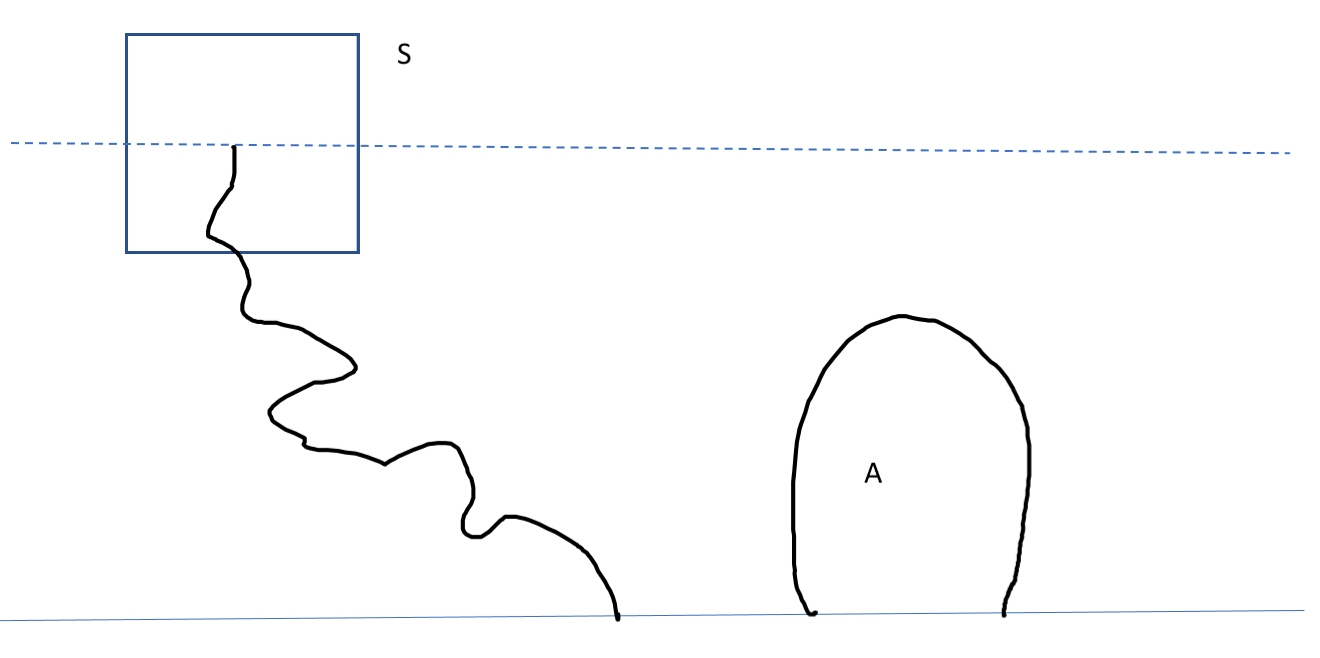
\includegraphics[scale=0.2]{7}
    \end{center}
\end{figure}

Then by a simple(?) symmetry argument,
\begin{align*}
& \prob_z [B(\eta) \in l] > 1/4, \\
& \prob_w [B(\eta)\in l] \leq 1/4,\quad \,\, \forall w\in S, \,\, \text{Im}(w) \leq r
\end{align*}
So
\begin{align*}
\frac{1}{4} &< \prob_z [B(\eta) \in l] \\
&= \prob_z [B(\eta) \in l, B[0, \eta] \cap \gamma[0, \sigma_r] = \phi] + \prob_z [B(\eta) \in l, B[0, \eta] \cap \gamma[0, \sigma_r] \neq \phi] \\
&= \prob_z[B(\eta) \in l \, | B[0, \eta] \cap \gamma[0, \sigma_r] = \phi] \prob_z[B[0, \eta]\cap \gamma[0, \sigma_r] = \phi] \\
& \quad + \prob_z [B(\eta)\in l \, | B[0,\eta] \cap \gamma[0, \sigma_r] \neq \phi] \prob_z[B[0,\eta] \cap \gamma[0, \sigma_r] \neq \phi]  
\end{align*}
Observe that the $\prob_z [B(\eta)\in l \,| B[0,\eta] \cap \gamma[0, \sigma_r] \neq \phi] \leq 1/4$, by the \emph{Strong Markov Property} of BM applied upon $B$ hits $\gamma[0, \sigma_r]$. Hence
\begin{align*}
& \prob_z [B(\eta) \in l \,| B[0, \eta] \cap \gamma[0, \sigma_r] =\phi] >\frac{1}{4} \\
\Rightarrow \quad & \text{(Denominator)} \geq \frac{1}{4} \prob_z [B[0, \eta]\cap \gamma[0, \sigma_r]=\phi] \times \frac{1}{R-r+1}
\end{align*}
where the factor $\frac{1}{R-r+1}$ comes from $\prob[\inf\{t\geq \eta : \text{Im}(B_t)= R\} \leq \inf\{t\geq \eta : \text{Im}(B_t)= r \} | B_{\eta} \in l]$ and is computed using the probability of a \emph{Gambler's Ruin}.
\s

Also, the \emph{Strong Markov Property} for $B$ at time $\eta$ and the \emph{Beurling estimate} implies (because we have assumed the hieght of $A$ is $\leq 1$, $B$ has to escape $D(B_{\eta}, r)$ before hitting $A$)
\begin{align*}
\prob_z [B\text{ hits }A\text{ before hitting } \reals\cup \gamma[0, \sigma_r]] \leq C r^{-1/2} \prob_z [B[0, \eta] \cap \gamma [0, \sigma_r] = \phi]
\end{align*}
So $\text{(Numerator)} \leq \frac{1}{R} Cr^{-1/2}$, with the factor $\frac{1}{R}$ comes from the probability that $B$ reaches hieght $R$ before hitting $\reals$, and is again computed using the probability of a \emph{Gambler's Ruin}. Putting the two estimates for the denominator and the numerator, we have the desired result.
\end{subproof}
This will finish claim 1 as 
\begin{align*}
\psi'_{\sigma_r} (U_{\sigma_r}) = \text{Probability that a Brownian excursion }\H\text{ from }U_{\sigma_r}\text{ to }\infty\text{ does not hit }g_{\sigma_r}(A)\\
=\text{Probaibilty that a Brownian excursion in }\H \backslash \gamma [0, \sigma_r]\text{ from }\gamma(\sigma_r)\text{ to }\infty\text{ does not hit }A. 
\end{align*}
So, we see that
\begin{align*}
1\geq \psi_{\sigma_r}'(U_{\sigma_r}) \geq 1- Cr^{-1/2} \rightarrow 1 \quad \text{as } r\rightarrow \infty
\end{align*}
This implies $M_{\sigma_r \wedge \tau} \rightarrow 1$ as $r \rightarrow \infty$ on $V_A$, and so $M_{t\wedge \tau} \rightarrow 1$ as $t \rightarrow 1$ on $V_A$ (as both limits have to be the same).   
\end{subproof}
\textbf{$\spadesuit$ Claim 2:} $M_{t\wedge \tau} \rightarrow 0$ as $t\rightarrow \infty$ on $V_A^c$.
\begin{subproof}
: Assume that $A$ is bounded by a smooth, simple curve $\beta : (0, 1) \rightarrow \H$ that is sufficiently close to $A$. (Will be justifying on \emph{Example Sheet \#2}). Note, because we are working on the event $V_A^c$, we have $\gamma(\tau) = \beta(s)$ for some $s\in (0,1)$. Since $\beta$ is a smooth, simple curve, there exists $\delta >0$ so that $l = [\beta(s), \beta(s) + \delta \vec{n}]\in $, where $\vec{n}$ is the inward pointing normal at $\beta(s)$.

\quad Let $l_t =g_t(l) -g_t(0)$, and $t_m = \inf\{t\geq 0 : |\gamma(t) -\beta(s)| \leq \frac{1}{m} \}$ for each $m\in \mathbb{N}$. We want to show that as $m\rightarrow \infty$, the probability that a Brownian excursion in $\H \backslash \gamma [0, t_m]$ from $\gamma(t_m)$ to $\infty$ hits $A \rightarrow 1$.

\quad Note, that the chance for a Brownian motion starting on any point on $l$ and hitting $\reals \cup \gamma [0, t_m]$ on either its left or right sides is bounded below by a strictly positive value. So
\begin{align*}
l_{t_m} \subset \{ w\in \H : \text{Im}(\omega) \geq a|\text{Re}(\omega)|\}
\end{align*}
for some $a>0$.

\quad In \emph{Example Sheet \#2}, will be showing that a Brownian excursion from 0 to $\infty$ in $\H$ hits $l_{t_m}$ with probability $\rightarrow 1$ as $m\rightarrow \infty$. So this implies that $\psi_{t}'(U_t) \rightarrow 0$ as $t\rightarrow \tau^-$. 
\end{subproof}
\eop
\end{p}
\s

In next two lectures, we are going to talk about more recent works on SLEs, including Gaussian free field(=``Random Mountain"). $\sle{4}$ curves describe the topographical map of the GFF. 
\s

\newday

(12th March, Tuesday)

\subsection*{The Gaussian free field (GFF)}

We have defined a Brownian motion $B: [0, \infty) \rightarrow \reals$ to be a ``random curve" indexed by time. We will define \emph{Gaussion free field (GFF)} $h: D\rightarrow \reals$ as a ``random filed" indexed by $D\subset \mathbb{C}$. This can be seen as a ``two-time dimensional analogue of Brownian motion". The construction would be based on the theory Hilbert spaces.
\s

\defi Let
\begin{align*}
C^{\infty} &= \{\text{functions on } \mathbb{C}\text{which are infinitely differentiable}\} \\
C_0^{\infty} &= \{f\in C^{\infty} \text{ with compact support}\} \\
C_0^{\infty}(D) &= \{f\in C_0^{\infty} \text{ with support }\subset D\}
\end{align*}
Suppose $f, g\in C_0^{\infty}$. Then the \textbf{Dirichlet inner product} of $f,g$ is
\begin{align*}
(f,g)_{\nabla} = \frac{1}{2\pi} \int \nabla f (x) \cdot \nabla(g) (x) dx
\end{align*}
\emph{[Poincar\'e's inequality ensures this is an inner product.]} Suppose that $D\subset \mathbb{C}$ is simply connected, but $D\neq \mathbb{C}$. Let $H_0^1(D)$=Hilbert space completion of $C_0^{\infty}(D)$ with respect to $(\cdot, \cdot)_{\nabla}$. Let $\snorms{f}{\nabla}^2 = (f,f)_{\nabla}$ be the norm on $H_0^1(D)$.

\subsubsection*{Propeerties of $H_0^1(D)$ and $(\cdot, \cdot)_{\nabla}$}

\begin{itemize}
\item[(1)] \textbf{Conformal invariance :} Suppose $\varphi : D \rightarrow \tilde{D}$ is a conformal transformation, $f, g\in C_0^{\infty}(D)$. Then
\begin{align*}
(f,g)_{\nabla} = (f\circ \varphi^{-1}, g\circ \varphi^{-1})_{\nabla}
\end{align*}
I other words, the Dirichlet inner product is conformally invariant. (The proof is on \emph{Ex Sheet \#2}.)

\quad This tells us that $H_0^1(D) \rightarrow H_0^1(\tilde{D})$ is given by $f \mapsto f\circ \varphi^{-1}$ is an isomrphism of Hilbert spaces.

\item[(2)] \textbf{Inclusion :} Suppose that $U\subset D$ is opne. If $f\in C_0^{\infty}(U)$, then $f\in C_0^{\infty}(D)$. Therefore we have a well-defined inclusion map $H_0^1(U) \hookrightarrow H_0^1(D)$. Therefore, $H_0^1(U)$ is a subspace of $H_0^1(D)$ 

\item[(3)] \textbf{Orthogonal decomposition :} For $U\subset D$ open, let $H_{\text{supp}}(U) = H_0^1(U) = H_0^1(U) \subset H_0^1(D)$ and $H_{\text{harm}}(U) = \{ f\in H_0^1(D) : f\text{ is harmonic on } U \}$. Then $H_0^1(D) = H_{\text{harm}}(U) \oplus H_{\text{supp}}(U)$ is an orthogonal decomposition.
\begin{p}
\pf To check orthogonality, suppose $f\in H_{\text{supp}}(U)$ and $g\in H_{\text{harm}}(U)$. Then
\begin{align*}
(f,g)_{\nabla} = \frac{1}{ 2\pi } \int \nabla f \cdot \nabla g = \frac{-1}{2\pi} \int f \lap g =0
\end{align*}

To see that they span $H_0^1(D)$, fix $f\in H_0^1(D)$. Let $f_0$ be the orthogonal projection $f$ onto $H_{\text{supp}}(U)$ and $g_0 = f- f_0$. We want $g_0$ to be harmonic on $U$. We will instead check that $g$ is `weakly harmonic'. Suppose $\varphi \in C_0^{\infty}(U)$. Then 
\begin{align*}
0 =(\varphi, g_0)_{\nabla} = \frac{1}{2\pi} \int \nabla \varphi \cdot \nabla g_0 = \frac{-1}{2\pi} \int (\lap \varphi) g_0 
\end{align*}
In \emph{Example Sheet \#2}, will check that this implies $g_0$ is harmonic on $U$ (and hence also $C^{\infty}$ on $U$).

\eop
\end{p}
\end{itemize}
\s

\subsubsection*{Definition of Gaussian free field}

Aside about normal random variables on $\reals^n$ :

Let $h= \alpha_1 e_1 + \cdots + \alpha_n e_n$ where $\alpha_1, \cdots, \alpha_n$ are iid $N(0,1)$ and $e_1,\cdots, e_n$ are standard basis on $\reals^n$. Then $h$ is a standard Gaussian random variable on $\reals^n$.
\begin{itemize}
\item If $x\in \reals^n$, then $(h, x) = \sum_{j=1}^n \alpha_j x_j \sim N(0, \snorms{x}{}^2)$.
\item If $x,y\in \reals^n$, then $(h,x)$, $(h,y)$ are jointly Gaussian with
\begin{align*}
\text{Cov}((h,x), (h,y)) = \sum_{j=1}^n x_j y_j = (x,y)
\end{align*}
\end{itemize}
So associated with $h$ is a \emph{family} of Gaussian random variables, $(h,x)$ indexed by $x\in \reals^n$ with covariance given by the standard inner product on $\reals^n$. This is an example of a \emph{Gaussian Hilbert space}.
\s

\defi Let $(f_n)$ be an orthonormal basis (ONB) of $H_0^1(D)$ and $(\alpha_n)$ be iid $N(0,1)$. Then $h$ on $D$ is given by
\begin{align*}
h = \sum_{n=1}^{\infty} \alpha_n f_n
\end{align*}
If $f= \sum_{n=1}^{\infty} \beta_n f_n \in H_0^1(D)$ for $\beta_n \in \reals$, then
\begin{align*}
(h, f)_{\nabla} = \sum_{n=1}^{\infty} \alpha_n \beta_n \sim N(0, \snorms{f}{\nabla}^2)
\end{align*}
If  $g= \sum_{n=1}^{\infty} \gamma_n f_n \in H_0^1(D)$, then $(h, f)_{\nabla}$, $(h,g)_{\nabla}$ are jointly Gaussian and $\text{Cov}((h,f)_{\nabla}, (h,g)_{\nabla}) = \sum_{n=1}^{\infty} \beta_n \gamma_n = (f,g)_{\nabla}$. The \textbf{Gaussian free field (GFF)} is a family of Gaussian random variables $(h,f)_{\nabla}$ indexed by $f\in H_0^1(D)$ with covariance given by $(\cdot, \cdot)_{\nabla}$.

\emph{[The expression $h =\sum_n \alpha_n f_n$ makes it seem like as if $h$ random varaible. Hoever, $h$ is not a function on $D$ as $\avg[\snorms{h}{D}^2] = \avg[\sum_{n=1}^{\infty} \alpha_n^2] = \infty$ and does not take finite value. It should rather be thought of as a collection of random variables.]}
\s

\subsubsection*{Properties of GFF}

\begin{itemize}
\item[(1)] \textbf{Conformally invariant :} if $\varphi : D \rightarrow \tilde{D}$ is a conformal transformation, $h = \sum_{n} \alpha_n f_n$ is a GFF on $D$, then $h\circ \varphi^{-1} = \sum_{n=1}^{\infty} \alpha_n f_n \circ \varphi^{-1}$ is a GFF on $\tilde{D}$.

\item[(2)] \textbf{Markov property :} if $U\subset D$ is open and $h$ is a GFF on $D$, then we can write $h= h_1 + h_2$ where $h_1$ is a GFF on $U$, $h_2$ is harmonic on $U$ and $h_1, h_2$ are independent. That is, if we are conditioned with the value of GFF outside of $U$, then the rest is just a GFF on $U$.
\begin{p}
\pf Choose the ONB $(f_n)$ for $H_0^1(D)$ to consist of an ONB $(f_n^1)$ of $H_{\text{supp}}(U)$ and $(f_n^2)$ of $H_{\text{harm}}(U)$. Then
\begin{align*}
h = \sum_{n} \alpha_n f_n = \sum_{n} \alpha_n^1 f_n^1 + \sum_n \alpha_n^2 f_n^2
\end{align*}
but $h_1 := \sum_{n} \alpha_n^1 f_n^1$ is a GFF in $U$ and $h_2 := \sum_{n} \alpha_n^2 f_n^2$ is harmonic in $U$.

\eop
\end{p}  
\end{itemize}

\subsubsection*{Analogue for Browanian Bridge}
\vspace{-10pt}

\begin{figure}[h]
    \begin{center}
    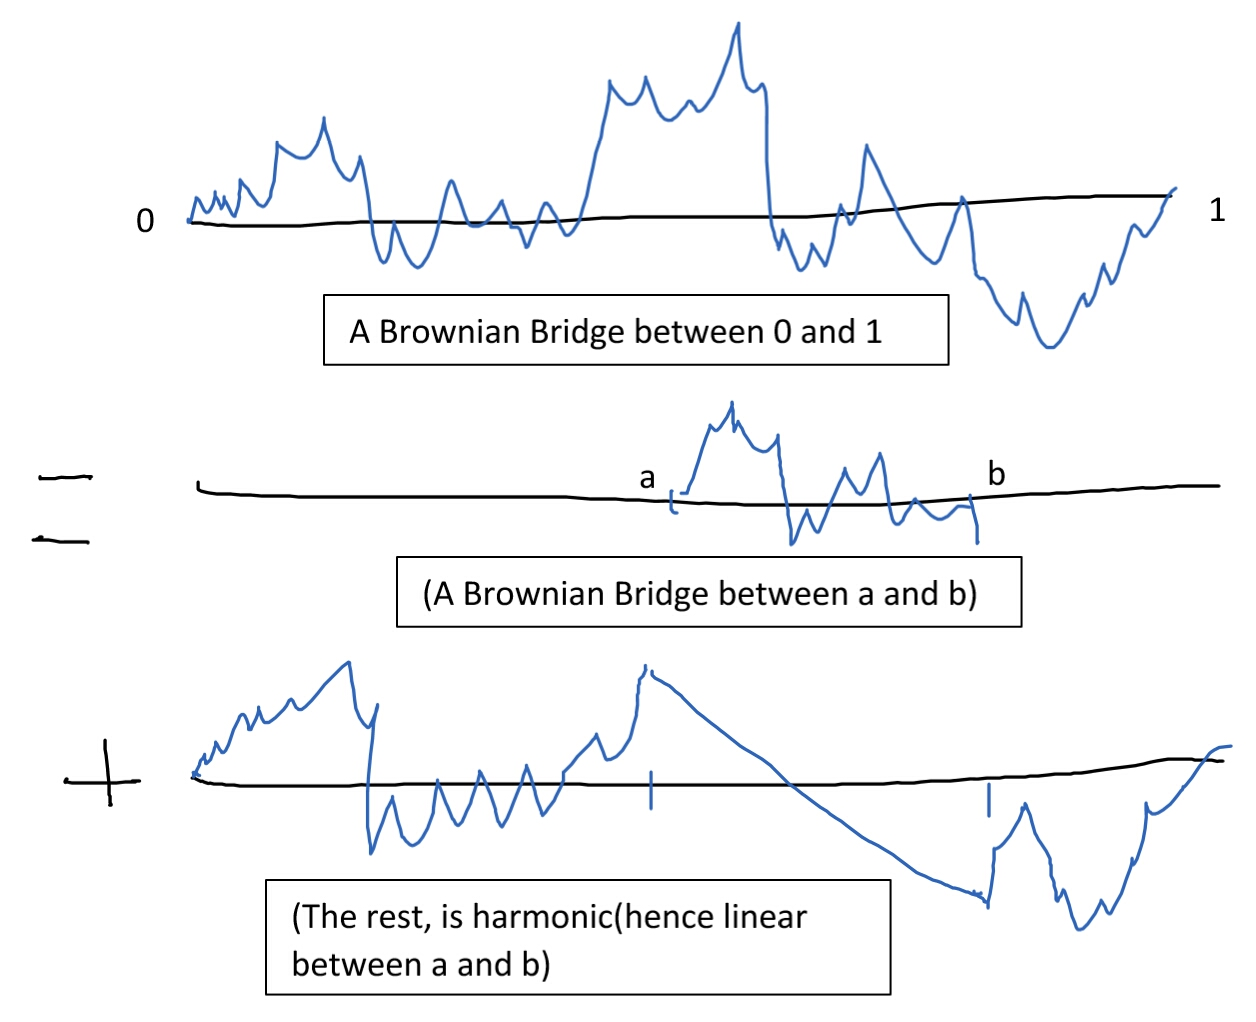
\includegraphics[scale=0.18]{8}
    \end{center}
\end{figure}
\s

\newday

(14th March, Thursday)

\subsubsection*{$L^2$ inner product of a $C_0^{\infty}$ function and the GFF}

Idea : if $h$ were a function then, we could have defined $(f,h) = -\frac{1}{2\pi} (h, \lap f)$. We would like to do something similar with distribution $h$.
\s

If $\varphi \in C_0^{\infty}(D)$, then we have 
\begin{align*}
-2\pi \lap^{-1} \varphi(x) = \int G(x,y) \varphi(y) dy
\end{align*}
where $G(x,y) = G_D(x,y) = -\log |x-y| -\tilde{G}_x(y)$ where $\tilde{G}_x(y)$ is harmonic in $D$ with boundary conditions $y\mapsto -\log |x-y|$ ($x$ fixed). $G= G_D$ is the \emph{Dirichlet Green's function} for $\lap$ on $D$.
\s

\textbf{Example :} When $D= \H$, has $G_{\H}(x,y) =-\log |x-y| + \log |x-\bar{y}|$.
\s

To define the $L^2$ inner product of $\varphi \in C_0^{\infty}$, we let
\begin{align*}
(h, \varphi) := (h, -2\pi \lap^{-1} \varphi) )_{\nabla}
\end{align*}
Thus $(h, \varphi)$ is a mean-zero normal random variable with variance
\begin{align*}
\text{Var}((h, \varphi)) &= \text{Var}((h, -2\pi \lap^{-1}\varphi)_{\nabla}) \\
&=(2\pi)^2 \snorms{\lap^{-1}\varphi}{\nabla}^2 = (2\pi)^2 (\lap^{-1}\varphi, \lap^{-1}\varphi)_{\nabla} \\
&= -2\pi (\lap^{-1}\varphi, \lap ( \lap^{-1} \varphi)) \quad \text{(integration by parts)} \\
&=\iint \varphi(x) G(x,y) \varphi(y)dxdx 
\end{align*}
Similarly
\begin{align*}
\text{Cov}((h, \varphi), (h, \psi)) = \iint \varphi(x) G(x,y) \psi(y) dxdy
\end{align*}
\s

\prop \emph{(Conformal invariance of the Grenns' fucntions)} If $D, \tilde{D} \subset \mathbb{C}$ are domains in $\mathbb{C}, \varphi : D \rightarrow \tilde{D}$ is a conformal transforamtion, then $G_D(x,y) = G_{\tilde{D}}(\varphi(x),\varphi(y))$. 
\begin{p}
\pf We have that, since confromal transformation preserves harmonicity, $G_D(x,y) - G_{\tilde{D}}(\varphi(x), \varphi(y))$ is harmonic on $D$. Also, it is clear from their deifinitions that $G_D(x,y) - G_{\tilde{D}}(\varphi(x), \varphi(y)) \equiv 0$ on the boundary, hence identically 0.

\eop 
\end{p}
\s

The GFF is not a function. It is a generalized function (a.k.a. a distribution). But speaking in the language of functions, we are going to see that `0-level sets' of the GFF $\{x: h(x) =0\}$ are described by $\sle{4}$ (Schramm, Sheffield).
\s

\thm Let $\lambda = \pi/2$. Let $\gamma$ be an $\sle{4}$ in $\H$ from $0$ to $\infty$, $(g_t)$ be its Loewner evolution, with $U_t =\sqrt{\kappa} B_t = 2B_t$ and $f_t = g_t - U_t$. Fix $U\subset \H$ open and let $\tau =\inf \{ t\geq 0 : \gamma(t) \in U \}$. Let $h$ be a GFF in $\H$, and $\hh = \lambda - \frac{2\lambda}{\pi} \text{arg}(\cdot)$. Then
\begin{align*}
h\circ f_{t\wedge \tau} + \hh \circ f_{t\wedge \tau} \xeq h + \hh
\end{align*}
where the left/right sides are restricted to $U$ (only integrate with respect to test functions supported in $U$).
\s

The theorem suggsets two different methods for sampliing a GFF.

\quad Let us think about the statement for a while. We will have
\begin{itemize}
\item $\hh = \text{harmonic in } \H\text{ with boundary condition }-\lambda$ on $\reals_-$, $+\lambda$ on $\real_+$.
\item $\hh \circ f_{t\wedge \tau}$=harmonic in $\H \backslash \gamma[0, t\wedge \tau]$ with boundary condtion $-\lambda$  on $\reals_-$ and left side of $\gamma[0, t\wedge \tau]$, $+ \lambda$ on $\reals_+$ and the right side of $\gamma[0, t\wedge \tau]$.
\item $\gamma$ is a ``level ridge" of $h$ (remind that $h$ is not a function)
\end{itemize}
This version of the theorem is a simplified from the original one. This theorem is not dealing with what happens after $\gamma$ hits $U$.
\s

\begin{p}
\pf Suppose $\phi \in C_0^{\infty} (U)$. We want to prove :
\begin{align*}
(h\circ f_{t\wedge \tau} + \hh \circ f_{t\wedge \tau}, \phi) \xeq (h+ \hh, \phi)
\end{align*}
\textit{i.e.} is $\sim N(m_0(\phi), \sigma_0^2(\phi))$ where $m_0(\phi) = (\hh, \phi)$, $\sigma_0^2 (\phi) = \iint \phi(x) G_{\H}(x,y) \phi(y) dxdy$. This is equivalent to showing
\begin{align*}
\avg\big[ \exp[ i\sigma(h\circ f_{t\wedge \tau} + \hh\circ f_{t\wedge \tau}) , \phi \big] = \exp \Big[i\theta m_0(\phi) - \frac{\theta^2}{2} \sigma_0^2(\phi) \Big]
\end{align*}
Let $\FF_t = \sigma(U_s : s\leq t)$. Given $\FF_{t\wedge \tau}$, $h\circ f_{t\wedge \tau}$ is a GFF in $\H \backslash \gamma[0, t\wedge \tau]$, so
\begin{align*}
& \avg [\exp( i\theta(h\circ f_{t\wedge \tau} + \hh\circ f_{t\wedge \tau} , \phi)) | \FF_{t\wedge \tau}]  \\
& = \avg \big[\exp (i\theta (h\circ f_{t\wedge \tau, \phi})) |\FF_{t\wedge \tau} \big] \exp \big[i\theta m_{t\wedge \tau}(\phi) \big] \\
& = \exp \Big(i\theta m_{t\wedge \tau}(\phi) - \frac{\theta^2}{2} \sigma_{t\wedge \tau}^2(\phi) \Big)
\end{align*}
where $\sigma_t^2 (\phi) = \iint \phi(x) G_t (x,y) \phi(y) dxdy$ with $G_t(x,y) = G_{\H}(f_t(x), f_t(y))$ is the Greens' function on $\H \backslash \gamma[0,t]$ and $m_t(\phi) := (\hh \circ f_t, \phi)$.

\quad We want to show that $\exp(i\theta m_t(\phi) - \frac{\theta^2}{2} \sigma_t^2(\phi))$ is a martingale. This is in the form of an exponential martingale, so showing $m_t(\phi)$ is a martingale with $[m_{\cdot}(\phi)]_t =\sigma_0^2(\phi) - \sigma_t^2(\phi)$ would be sufficient for this.
\begin{i}
\item Check that $m_t(\phi)$ is a martingale (recall $m_t(\phi) = (\hh \circ f_t, \phi)$):
\begin{align*}
\hh \circ f_t(z) &= \lambda - \frac{2\lambda}{\pi} \text{arg}(f_t(z)) \\
& = \lambda - \frac{2\lambda}{\pi} \text{Im}(\log(g_t(z) - U_t)) = \lambda - \text{Im}(\log(g_t(z) - U_t))
\end{align*}
We want to see that $\log(g_t(z) - U_t)$ is a martingale. To see this,
\begin{align*}
d\log (g_t(z) - U_t) &= \frac{1}{g_t(z) -U_t} \cdot \frac{2}{g_t(z) - U_t} dt - \frac{1}{g_t(z) - U_t} dU_t - \frac{\kappa/2}{(g_t(z) - U_t)^2} dt \\
& =\frac{2- \kappa/2}{(g_t(z) -U_t)^2}dt - \frac{2}{g_t(z) - U_t}dB_t = \frac{-2}{g_t(z) - U_t}dB_t
\end{align*}
since $\kappa =4$. So $m_t(\phi)$ is a martingale.

\item The quadratic variation is, by \emph{It\^o isometry},
\begin{align*}
d[m_{\cdot}(\phi)]_t = \iint \phi(z) \text{Im}(\frac{2}{g_t(z)- U_t}) \text{Im}(\frac{2}{g_t(w)- U_t})\phi(w) dzdw
\end{align*}
It will be enougth to show that $d\sigma_t^2(\phi)$ has the same form. To see this, observe
\begin{align*}
G_{\H}(z,w) &= - \text{Re}(\log(z-w) - \log(z-\bar{w})) \\
\log (f_t(z) - f_t(w)) &= \log (g_t(z) - g_t(w)) \quad (\text{used }f_t = g_t- U_t)
\end{align*}
so
\begin{align*}
d \log (g_t(z) - g_t(w)) &= \frac{1}{g_t(z) - g_t(w)} \cdot \Big( \frac{2}{g_t(z) - U_t} -\frac{2}{g_t(w)-U_t} \Big) dt \\
&=\frac{-2dt}{(g_t(z) - U_t)(g_t(w) - U_t)}
\end{align*}
and similarly
\begin{align*}
d\log (g_t(z) - \overline{g_t(w)}) = \frac{-2dt}{(g_t(z) - U_t)(\overline{g_t(w)} - U_t)}
\end{align*}
Hence, using conformal invariance of Green's function,
\begin{align*}
& dG_t(z,w) = -\text{Im}\Big( \frac{2}{g_t(z) - U_t} \Big) \text{Im}\Big(\frac{2}{g_t(w) - U_t} \Big) \\
\Rightarrow \quad & d\sigma_t^2(\phi) = \Big[ -\iint \phi(z) \text{Im}\big(\frac{2}{g_t(z) - U_t}\big) \text{Im}\big(\frac{2}{g_t(w) - U_t}\big) \phi(w) dzdw\Big]dt
\end{align*}
after some computation. so indeed $d[m_{\cdot}(\phi)]_t = d\sigma_t^2(\phi)$.
\end{i} 
These complete the proof.

\eop
\end{p}





\end{document}
